% Εκτύπωση σε χαρτί A4, μία σελίδα ανά φύλλο, με ξεχωριστή σελίδα για τον τίτλο,
% σε γραμματοσειρά 11pt και format άρθρου.
\documentclass[a4paper,oneside, 11pt]{article}
\usepackage[margin=0.7in]{geometry}

% Προσοχή στο [cm-default], χωρίς αυτό μπορεί να μην λειτουργούν τα
% μαθηματικά σύμβολα σε ορισμένες εγκαταστάσεις του xelatex!
\usepackage[cm-default]{fontspec}
\usepackage{xunicode}
\usepackage{xltxtra}
\usepackage{float}
\usepackage{mathtools}
\DeclarePairedDelimiter{\ceil}{\lceil}{\rceil}
\DeclarePairedDelimiter{\floor}{\lfloor}{\rfloor}
% Ελληνικό Hyphenation, αφαιρέστε το αν δεν έχετε εγκατεστημένο το xgreek.
\usepackage{xgreek}
\usepackage{listings}
\lstset{basicstyle=\footnotesize\ttfamily,breaklines=true}


% Γραμματοσειρά
\setmainfont[Mapping=tex-text]{CMU Serif}

% Χρήσιμο πακέτο για εισαγωγή εικόνων jpg/png ή άλλων εγγράφων pdf.
\usepackage{graphicx}
\usepackage{color}
 
\definecolor{codegreen}{rgb}{0,0.6,0}
\definecolor{codegray}{rgb}{0.5,0.5,0.5}
\definecolor{codepurple}{rgb}{0.58,0,0.82}
\definecolor{backcolour}{rgb}{0.95,0.95,0.92}
\usepackage{amsmath}


\lstdefinestyle{mystyle}{
    backgroundcolor=\color{backcolour},   
    commentstyle=\color{codegreen},
    keywordstyle=\color{magenta},
    numberstyle=\tiny\color{codegray},
    stringstyle=\color{codepurple},
    basicstyle=\footnotesize,
    breakatwhitespace=false,         
    breaklines=true,                 
    captionpos=b,                    
    keepspaces=true,                 
    numbers=left,                    
    numbersep=5pt,                  
    showspaces=false,                
    showstringspaces=false,
    showtabs=false,                  
    tabsize=2
}
 
\lstset{style=mystyle}

% Macro που δίνει το μέγιστο επιτρεπτό μέγεθος σε μια εικόνα,
% χωρίς να παραβιάζει τα όρια του LaTeX.
\makeatletter
\def\maxwidth{%
  \ifdim\Gin@nat@width>\linewidth
    \linewidth
  \else
    \Gin@nat@width
  \fi
}
\makeatother

% Ενεργοποιήστε την ακόλουθη γραμμή αν δεν θέλετε στοίχιση στις νέες παραγράφους.
%\parindent=0in


\title{\textbf{Bάσεις Δεδομένων Εξαμηνιαία Εργασία}}
\author{ Ιωάννης Δάρας (03115018 - \texttt{daras.giannhs@gmail.com}) \\ 
Μαρία Παρέλλη (03115155 - \texttt{maryparelli@gmail.com } ) }
\date{"The great advantage of a hotel is that it is a refuge from home life." \\
- George Bernard Shaw}

\begin{document}
\maketitle

\section{Οργάνωση κώδικα και δομή ιστοσελίδας}
Στην παρούσα ενότητα περιγράφεται η οργάνωση του κώδικα και η δομή της ιστοσελίδας όπως αυτή προκύπτει από τις μεταβάσεις μεταξύ των διαφορετικών παρεχόμενων οθονών.
\subsection{Οργάνωση κώδικα}
Κάνοντας unzip το αρχείο που έχει υποβληθεί στο mycourses βλέπουμε τους εξής φακέλους:
\begin{enumerate}
\item ./report/ : Περιέχει τα αρχεία για την ανάπτυξη της παρούσας αναφοράς σε \LaTeX καθώς και ένα export της σε pdf.
\item WebContent: Περιέχει το front-end της εφαρμογής. Ειδικότερα:
\begin{enumerate}
\item ./WebContent/bootstrap : Περιέχεται ο κώδικας του bootstrap framework που χρησιμοποιείται σε μεγάλο βαθμό (ιδιαίτερα το grid system που παρέχει) για το σχεδιασμό του css της εφαρμογής.
\item ./WebContent/fancy\_table: Περιέχει μια υλοποίηση βασισμένη σε Javascript και css ενός διαδραστικού table που χρησιμοποιούμε στην εφαρμογή μας.
\item ./WebContent/favicons : Περιέχει το fontawesome που χρησιμοποιείται για διάφορα favicons της εφαρμογής μας.
\item ./WebContent/images : Περιέχει το background image αλλά και διάφορες άλλες εικόνες που χρησιμοποιούμε σε διάφορα σημεία στην εφαρμογή μας.
\item ./WebContent/js : περιέχει το calender.js που πρακτικά είναι ένα custom ημερολόγιο που χρησιμοποιούμε για την επιλογή των start και finish dates στην εφαρμογή μας.
\item ./WebContent/META-INF : περιέχει το manifest της εφαρμογής μας
\item ./WebContent/WEB-INF : περιέχει διαθέσιμες βιβλιοθήκες αλλά και το αρχείο web.xml που χρησιμεύει ως config file για την εφαρμογή μας.
\item ./WebContent/*.jsp : Τα αρχεία αυτά αποτελούν τις σελίδες της εφαρμογής μας.
\item ./WebContent/theme.css : περιέχει το css template που γράψαμε για την εφαρμογή μας.
\end{enumerate}
\item ./src/com/ntua/databases/ : Στον φάκελο αυτό συναντάμε τα εξής αρχεία:
\begin{enumerate}
\item ./src/com/ntua/databases/Connector.java : αποτελεί το αρχείο που μας εξασφαλίζει τη σύνδεση με τη βάση δεδομένων
\item Διάφορα Servlets : Τα Servlets αυτά είναι Java αρχεία που επικοινωνούν με τη βάση (την ρωτάνε, τροποποιούν τα δεδομένα της, τα διαγράφουν, κ.α.) ανάλογα με τις εισόδους που βάζει στις αντίστοιχες φόρμες ο χρήστης. Στη συνέχεια, τα αποτελέσματα τους τα επιστρέφουν στα jsp files. Σημειώνεται ότι τα servlet χρησιμοποιούνται και για form validation.
\end{enumerate}
\item ./src/com/ntuadatabases/ : Εδώ συναντάμε Servlets που αφορούν το κομμάτι του administration της βάσης δεδομένων. Συγκεκριμένα, έχουμε:
\begin{enumerate}
\item ./src/com/ntuadatabases/controller/ : Οι controllers για την ανταλλαγή πληροφοριών μεταξύ Servlet και jsp files.
\item ./src/com/ntuadatabases/dao/ : Εδώ βρίσκονται Java files που ρωτάνε ή τροποποιούν το κομμάτι της βάσης που αφορά το database administration.
\item ./src/com/ntuadatabases/model/ : Εδώ ορίζονται μοντέλα (κλάσσεις) των οποίων τα instances περνάμε στα jsp files μέσω των controllers.
\end{enumerate}
\item ./build : Εδώ βρίσκονται τα build files της εφαρμογής μας.
\item ./database-setup : Εδώ βρίσκονται τα ακόλουθα αρχεία:
\begin{enumerate}
\item ./database-setup/tables-creator : sql script που δημιουργεί όλους τους πίνακες στη βάση δεδομένων μας.
\item ./database-setup/database-initializer : sql script που αρχικοποιεί τη βάση δεδομένων μας με διάφορα δεδομένα.
\item ./database-setup/database-triggers.sql : sql script που περιέχει τους triggers της βάσης μας.
\item .database-setup/database-indexes.sql : sql script που ορίζει ευρετήρια για τη βάση μας.
\item .database-setup/database-views.sql : Εδώ ορίζονται όψεις της βάσης δεδομένων μας.

\item ./LICENCE : περιέχει την άδεια της εφαρμογης 
\item ./README.md : περιέχει το README file της εφαρμογής όπως αυτό πάρθηκε από το repository της ομάδας στο Github.
\end{enumerate}
\end{enumerate}
\subsection{Δομή Ιστοσελίδας - Μεταβάσεις}
H αρχική σελίδα της εφαρμογής μας είναι το welcome.jsp, στο οποίο υπάρχουν 3 κουμπιά, το καθένα από τα οποία αντιστοιχεί σε μία από τις τρεις κατηγορίες χρηστών της εφαρμογής μας:
\begin{figure}[h]
\center
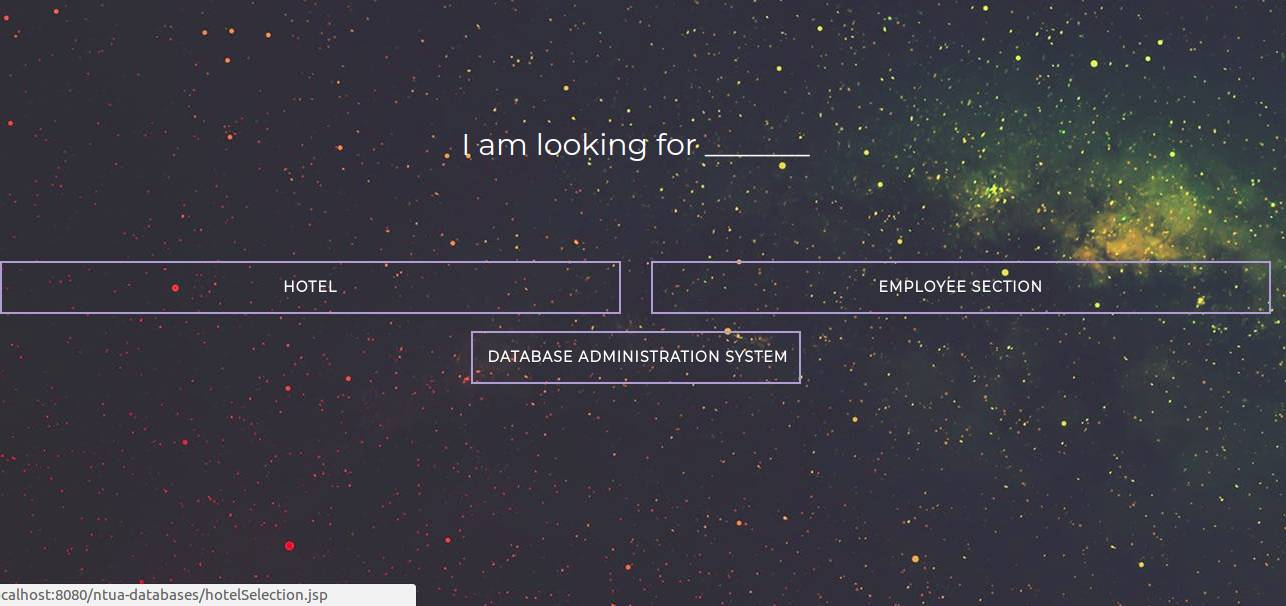
\includegraphics[width=0.9\textwidth]{welcome.jpg}
\end{figure}

\begin{enumerate}
\item Hotel: το επιλέγουν οι πελάτες των ξενοδοχείων για να μεταβούν στη σελίδα hotelSelection.jsp, όπου θα θέσουν τα κριτήρια τους για την αναζήτηση ξενοδοχείου.
\item Employee Login:το επιλέγουν οι ενεργοί υπάλληλοι των ξενοδοχειών για να μεταβούν στην σελίδα EmployeeLogin.jsp, όπου γίνεται επιβεβαίωση της ταυτότητας τους.
\item Database Administration System:το επιλέγει ο διαχειριστής της βάσης για να μεταβεί στη σελίδα protectedLogin.jsp, όπου θα εισάγει τον ειδικό κωδικό ώστε να αποκτήσει πρόσβαση στις λειτουργίες της βάσης δεδομένων.
\end{enumerate}

Συνεπώς εξάγουμε το συμπέρασμα ότι ανάλογα με το ποιος χρησιμοποιεί την ιστοσελίδα μας διαμορφώνονται 3 ξεχωριστές διαδρομές:

\begin{enumerate}
\item \textbf{Διαδρομή πελάτη} \bigbreak
Αφού ο πελάτης επιλέξει το κουμπί Hotel στην αρχική σελίδα,οδηγείται στη σελίδα 		hotelSelection.jsp,όπου θέτει τα κριτήρια για την επιλογή δωματίων. Συγκεκριμένα, μπορεί να επιλέξει κατηγορία ξενοδοχείου,αριθμό δωματίων,περιοχή,ημερομηνίες καθώς και όμιλο,στον οποίον θέλει να ανήκει.
\begin{figure}[h]
\center
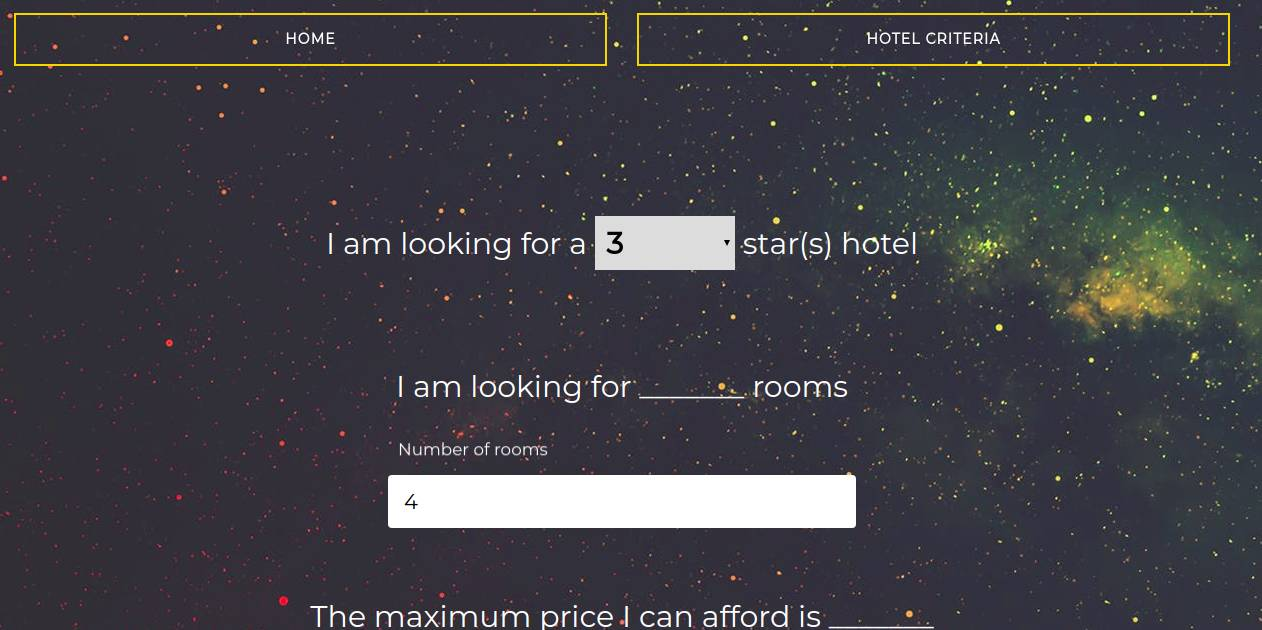
\includegraphics[width=0.9\textwidth]{hotelSel1.jpg}
\end{figure}

Φυσικά, του δίνεται η επιλογή να προσαρμόσει την αναζήτηση του συμπληρώνοντας όσα από τα παραπάνω κριτήρια επιθυμεί. Παράλληλα,του δίνεται η επιλογή να λάβει τα δωμάτια ταξινομημένα  ανά κατηγορία είτε ανά περιοχή.
Στη σελίδα αυτή δίνεται η δυνατότητα στον πελάτη να δει και τις όψεις της βάσης που αφορούν τον αριθμό των διαθέσιμων δωματίων ανά περιοχή και τον αριθμό των διαθέσιμων δωματίων ανά capacity.

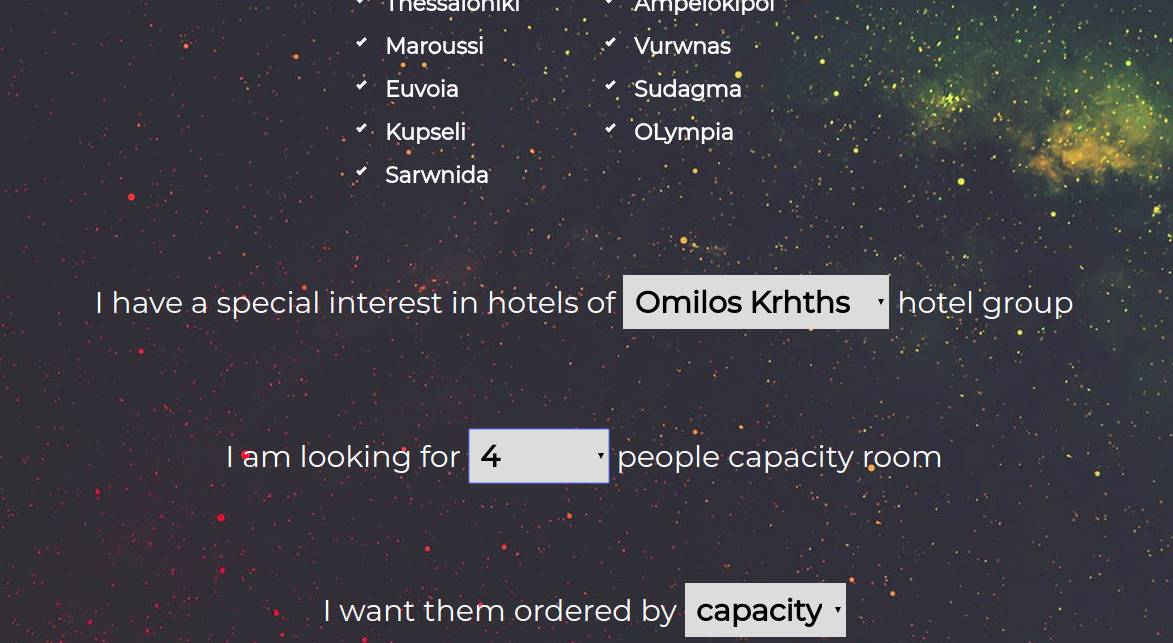
\includegraphics[width=0.9\textwidth]{hotelSel2.jpg}
\bigbreak
Πατώντας του κουμπί Query Me, ο χρήστης πραγματοποιεί την αναζήτηση. 
Αυτό επιτυγχάνεται ώς εξής: \bigbreak Τα πεδία, τα οποία συμπλήρωσε ο χρήστης στέλνονται ώς παράμετροι στο servlet SearchServlet.java ,όπου γίνονται τα κατάλληλα queries στη βάσ και τα αποτελέσματα στέλνονται στη σελίδα roomselection.jsp. Στη σελίδα αυτή ο χρήστης μπορεί να δει τα χαρακτηριστικά και να επιλέξει ανάμεσα στα δωμάτια,που πληρούν τις προϋποθέσεις , που εισήγαγε. 

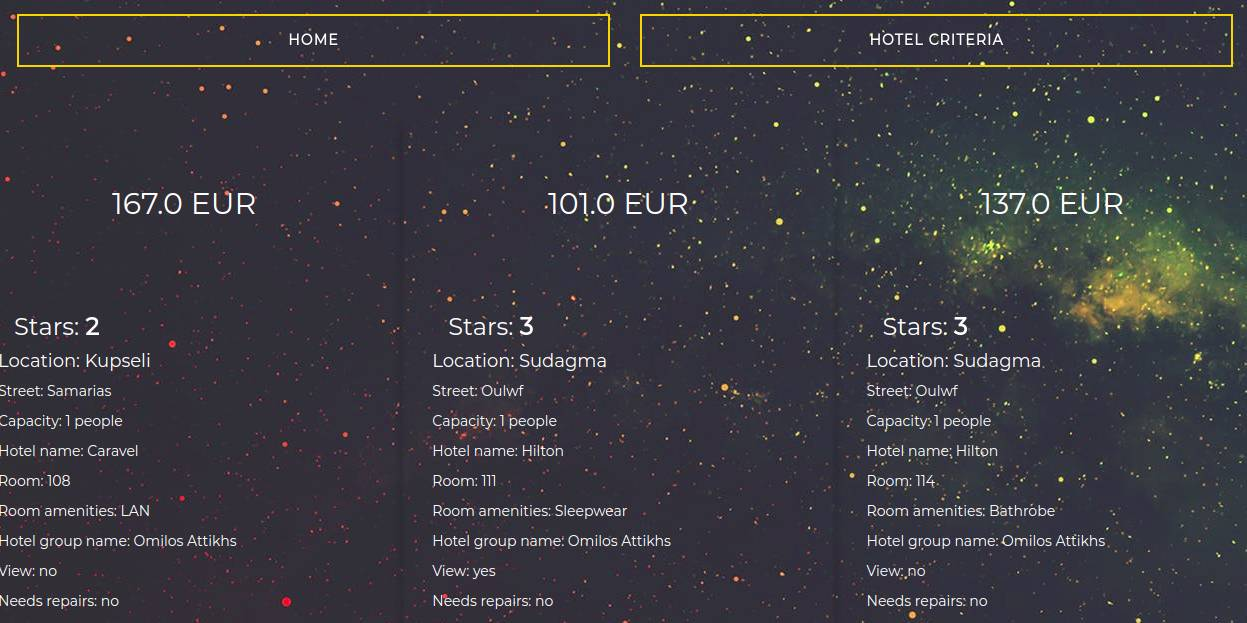
\includegraphics[width=0.9\textwidth]{roomSel.jpg}
\bigbreak


Μόλις επιλέξει το δωμάτιο, που επιθυμεί  μεταφέρεται στη σελίδα identifyCustomer.jsp, όπου του ζητείται να επιβεβαιώσει την ταυτότητα του δίνοντας το ΑΦΜ του. Έαν δεν υπάρχει στη βάση πελάτης καταχωρημένος με αυτό το ΑΦΜ,τότε ο πελάτης ανακατευθύνεται στη σελίδα createCustomer.jsp, στην οποία εισάγει τα στοιχεία του και δημιουργείται ο λογαριασμός του. Αντίθετα, εάν ο πελάτης είναι καταχωρημένος στη βάση τότε κατευθύνεται στη σελίδα reservationDates.jsp, στην οποία εισάγει της ημερομηνίες, στις οποίες επιθυμεί να γίνει η κράτηση. Εάν το δωμάτιο είναι ακόμη διαθέσιμο, τότε η κράτηση πραγματοποιείται με επιτυχία και ο πελάτης μεταφέρεται στη σελίδα reservationReady.jsp. Σε αντίθετη περίπτωση μεταφέρεται στη σελίδα reservationProblem.jsp.
\begin{figure}[h]
\center
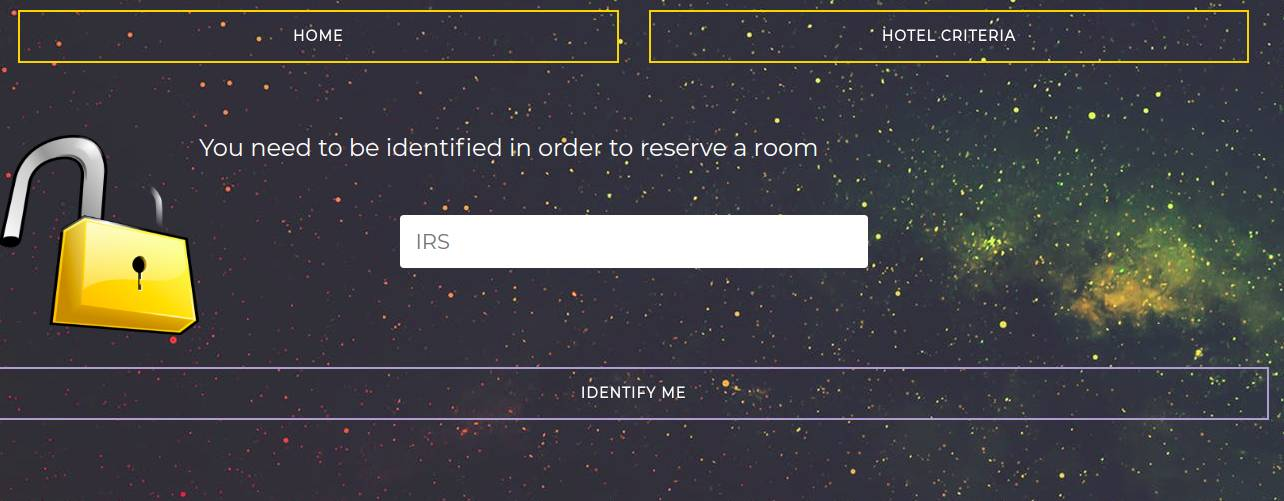
\includegraphics[width=0.9\textwidth]{identify.jpg}
\bigbreak
\end{figure}



Όλα τα παραπάνω σε επίπεδο εφαρμογής πραγματοποιούνται ώς εξής: Όταν ο χρήστης επιλέξει δωμάτιο τα στοιχεία room\_id,hotel\_id,δηλαδή τα πρωτεύοντα κλειδιά της σχέσης hotel\_room περνούν ώς παράμετροι στο servlet IdentifyCustomer.java. Εκεί γινεται query στη σχέση customer, για να διαπιστωθεί εάν ο πελάτης υπάρχει στη βάση.Ανάλογα με το αποτέλεσμα ο χρήστης κατευθύνεται και στην αντίστοιχη σελίδα, όπως αναλύθηκε παραπάνω. Εάν ο πελάτης υπάρχει, στη σελίδα reservationDates.jsp μεταφέρονται ως παράμετροι το room\_id,το hotel\_id,το ΑΦΜ του πελάτη καθώς και το ονοματεπώνυμό του. Εάν ο πελάτης δεν υπάρχει,κατευθύνεται στη σελίδα createCustomer.jsp, όπου μεταφέρονται ως παράμετροι, το room\_id,το hotel\_id καθώς και το ΑΦΜ του. Τα πεδία, που ο πελάτης συμπληρώνει στη σελίδα στέλνονται στο servlet NewCustomer.java,όπου γίνονται οι κατάλληλες εισαγωγές στη βάση και ο έλεγχος μεταφέρεται στη σελίδα reservationDates.jsp.

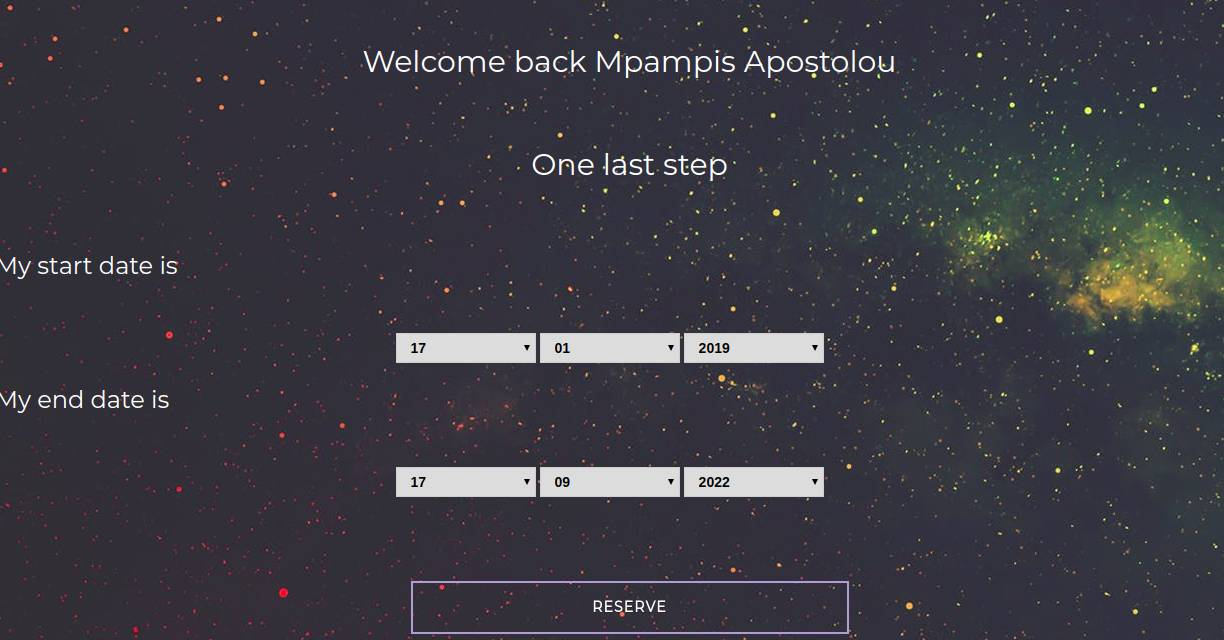
\includegraphics[width=0.9\textwidth]{reserve.jpg}
\bigbreak

Aφού ο πελάτης εισάγει τις επιθυμητές ημερομηνίες για το δωμάτιο της επιλογής του, αυτές μεταφέρονται ως παράμετροι στο servlet Reservation.java, στο οποίο γίνεται έλεγχος εάν στο δωμάτιο αυτό έχει εντωμεταξύ γίνει κράτηση για τις ίδιες ημερομηνίες. Eάν όχι γίνεται η κατάλληλη εισαγωγή στη σχέση reserves και ο έλεγχος μεταφέρεται στη σελίδα reservationReady.jsp. Εάν ναι,τότε ο έλεγχος μεταφέρεται στη σελίδα reservationProblem.jsp.


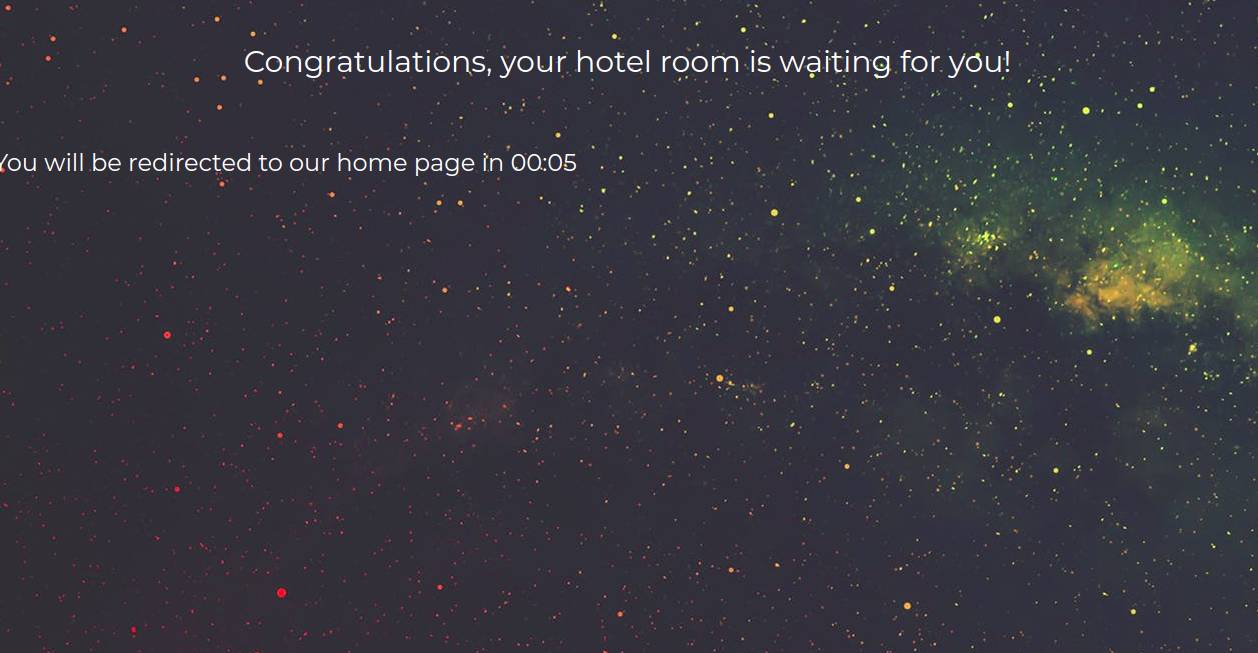
\includegraphics[width=0.9\textwidth]{success.jpg}
\bigbreak

\item \textbf{Διαδρομή υπαλλήλου}

Ο υπάλληλος ξενοδοχείου στη σελίδα welcome.jsp επιλέγει το κουμπί Employee Section και μεταφέρεται στη σελίδα EmployeeLogin.jsp,στην οποία εισάγει το ΑΦΜ του.Εάν αυτό αντιστοιχεί σε πεδίο στη βάση Employee, τότε η σύνδεση του είναι επιτυχής και μεταφέρεται στη σελίδα employeeRent.jsp. Aντίθετα εμφανίζεται μήνυμα λάθους. Στη σελίδα employeeRent.jsp ο υπάλληλος,μπορεί να δεί τις ανοιχτές κρατήσεις για τα ξενοδοχείο, στο οποίο εργάζεται. 

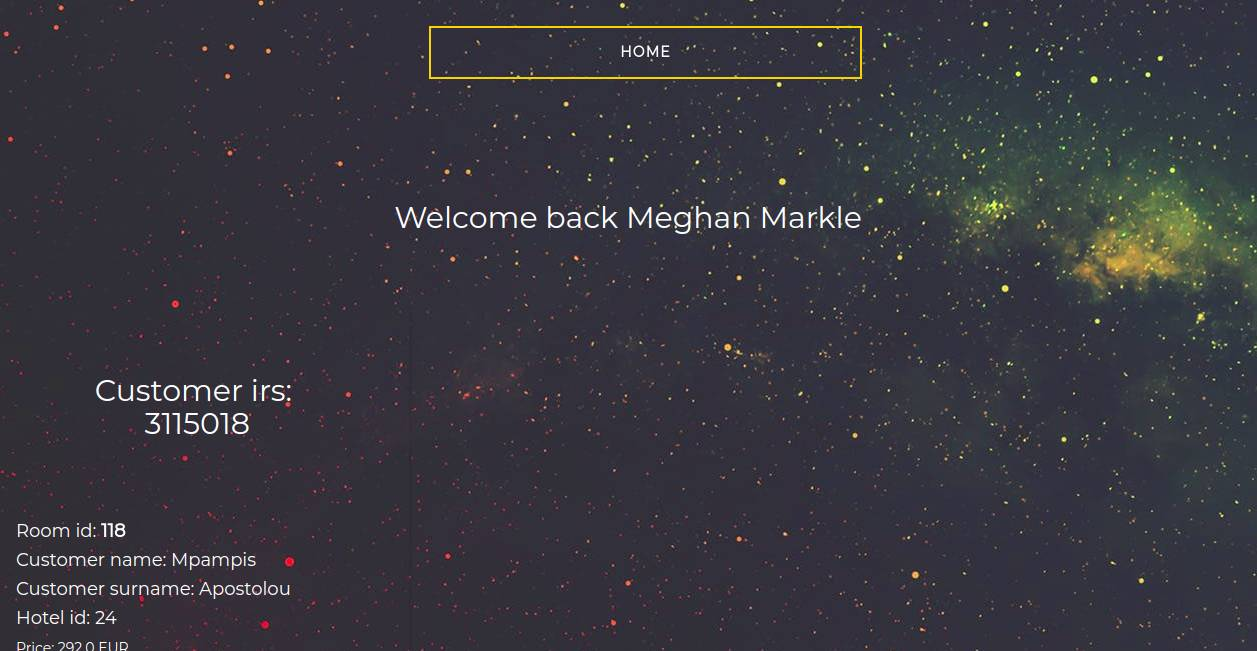
\includegraphics[width=0.9\textwidth]{rent.jpg}
\bigbreak
Όταν απαιτηθεί να γίνει το check-in του πελάτη ο υπάλληλος επιλέγει την κράτηση,που του αντιστοιχεί και μεταφέρεται στη σελίδα implementPayment.jsp. Στη σελίδα αυτή ο υπάλληλος εισάγει μέθοδο πληρωμής και μόλις πραγματοποιηθεί με επιτυχία η ενοικίαση ο υπάλληλος μεταφέρεται πίσω στη σελίδα employeeRent.jsp, για να δεί και τις υπόλοιπες διαθέσιμες κρατήσεις.
\bigbreak
Σε επίπεδο εφαρμογής τα παραπάνω πραγματοποιούνται ως εξής:Όταν ο υπάλληλος εισάγει το ΑΦΜ του αυτό περνάται ως παράμετρος στο servlet IdentifyEmployee,java, στο οποίο γίνεται query στη σχέση employee, για να διαπιστωθεί εάν ο υπάλληλος είναι καταχωρημένος στη βάση. Στη συνέχεια, γίνονται τα κατάλληλα queries στις σχέσεις reserves, hotel\_room και customer, ώστε τα δεδομένα για τις διαθέσιμες κρατήσεις στο ξενοδοχείο εργασίας του υπαλλήλου να περαστούν στη σελίδα EmployeeRent.jsp. Αφού ο υπάλληλος επιλέξει τη κράτηση του πελάτη,ο οποίος πραγματοποιεί το check-in και εισάγει μέθοδο πληρωμής στη σελίδα implementPayment.jsp, τα δεδομένα της ενοικίασης (room, hotel,price, irs\_employee,i rs\_customer,start\_date,finish\_date,payment\_amount,payment\_method) στέλνονται στο servlet RentServlet.java.Στο servlet αυτό γίνεται η κατάλληλη εισαγωγή στη σχέση rents και στη συνέχεια ο έλεγχος μεταφέρεται στη σελίδα IdentifyEmployee.jsp.

\item \textbf{Διαδρομή διαχειριστή βάσης} \bigbreak 
Ο διαχειριστής της βάσης στη σελίδα welcome.jsp  επιλέγει το κουμπί Database Administration System και μεταφέρεται στη σελίδα protectedLogin.jsp. 
\begin{figure}[h]
\center
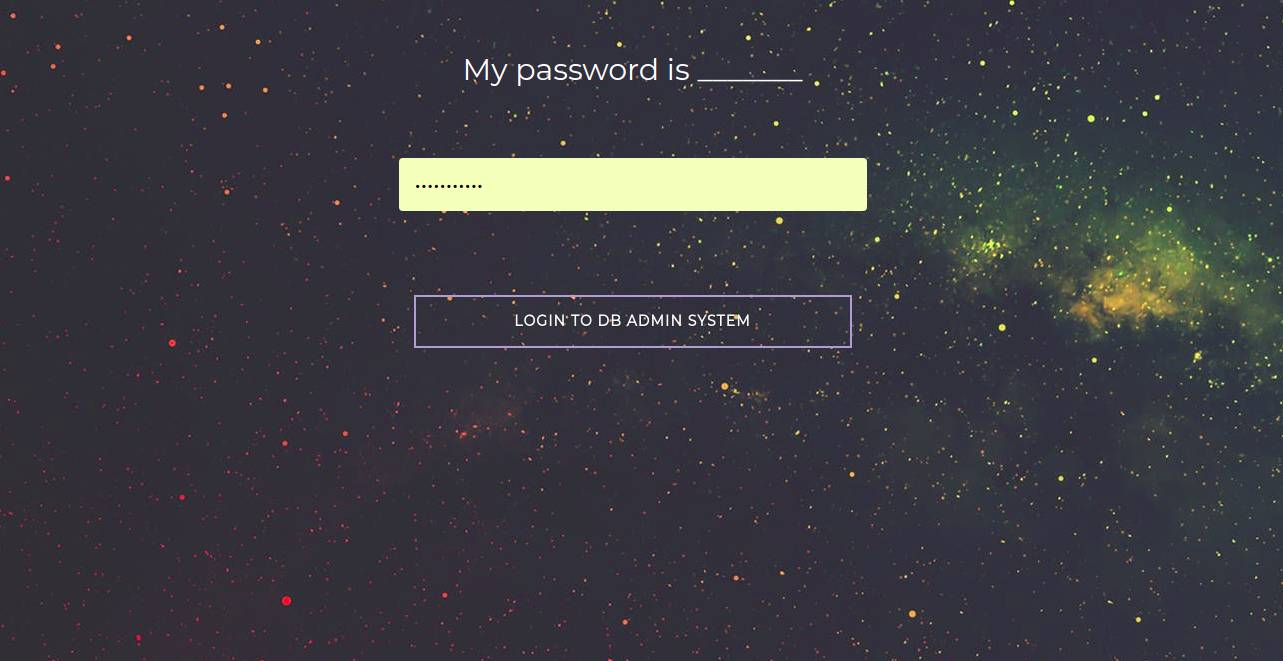
\includegraphics[width=0.9\textwidth]{adminpass.jpg}
\bigbreak
\end{figure}

Εκεί εισάγει τον κωδικό του, ο οποίος στη συνέχεια μεταφέρεται ώς παράμετρος στο servlet Checker.java και ελέγχεται η ορθότητα του. Αν είναι έγκυρος, ο διαχειριστής μεταφέρεται στη σελίδα Administratorpage,όπου επιλέγει ποιο πίνακα επιθυμεί να επεξεργαστεί. Οι επιλογές, που του παρέχονται είναι: hotels,hotel\_groups και rooms.

\begin{figure}[h]
\center
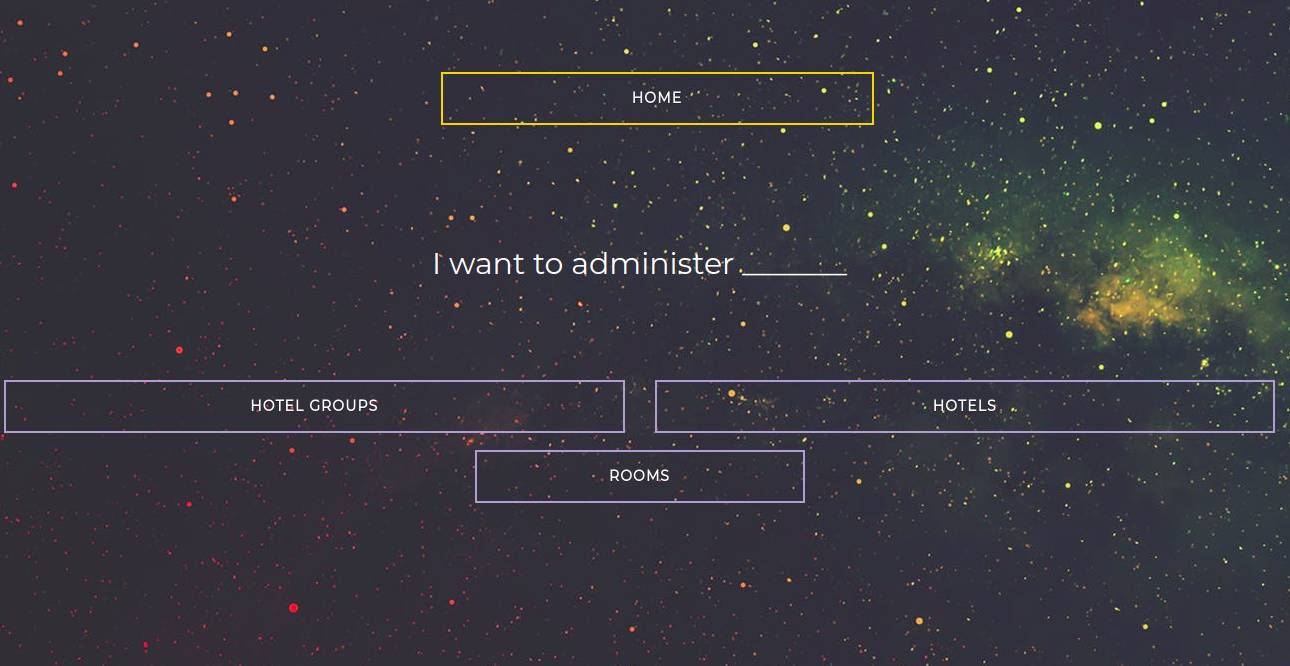
\includegraphics[width=0.9\textwidth]{admin.jpg}
\bigbreak
\end{figure}

\begin{itemize}
\item Hotel groups. \bigbreak 
Εάν επιλέξει hotel groups μεταφέρεται στη σελίδα listadminhotelgroups.jsp, όπου του εμφανίζεται ένας πίνακας με όλες τις εγγραφές της σχέσης hotel\_group. Αυτό γίνεται εφικτό μέσω του servlet Hotelgroupscontroller.java δίνωντας του ώς παράμετρο action=listhotelgroups. Δίπλα σε κάθε εγγραφή,υπάρχει η επιλογή να τη διαγράψει ή να την επεξεργαστεί. Eπιπλέον, υπάρχει στο πάνω μέρος της οθόνης κουμπί,το οποίο επιλέγει για να προσθέσει νέα εγγραφή. Εάν επιλεγεί να προστεθεί η να ανανεωθεί εγγραφή, ο διαχειριστής μεταφέρεται στη σελίδα adminhotelgroups.jsp, όπου συμπληρώνει τα κατάλληλα πεδία και στη συνέχεια  οι τιμές τους περνάνε ώς παράμετροι στο hotelgroupscontroller και γίνεται αντίστοιχα προσθήκη η ανανέωση στη σχέση hotel\_groups. Ομοίως, εάν επιλεγεί διαγραφή πεδίου, το hotel\_group\_id περνάται ως παράμετρος στο servlet μαζί με action=delete,όπου και πραγματοποιείται η διαγραφή του πεδίου. \bigbreak 
Επιπλέον,δίπλα σε κάθε εγγραφή δίνεται επιλογή list\_emails και list\_phones,όπου μέσω του servlet Hotelgroupmailscontroller και Hotelgroupphonescontroller αντίστοιχα  και δίνοντας τους τις κατάλληλες παραμέτρους και actions ο διαχειριστής μπορεί να δεί σε λίστα τις εγγραφές στους πίνακες hotel\_group\_mails και hotel\_group\_phones, να τις διαγράψει ή να προσθέσει νέες.

\item Hotels. \bigbreak 
Εάν επιλέξει hotels ακολουθείται παρόμοια διαδικασία. Ο διαχειριστής μεταφέρεται στη σελίδα listadminhotels.jsp, όπου του εμφανίζεται ένας πίνακας με όλες τις εγγραφές της σχέσης hotel. Αυτό γίνεται εφικτό μέσω του servlet Hotelscontroller.java δίνoντας του ώς παράμετρο action=listhotelgroups. Δίπλα σε κάθε εγγραφή,υπάρχει η επιλογή να τη διαγράψει ή να την επεξεργαστεί. Επιπλέον,υπάρχει στο πάνω μέρος της οθόνης κουμπί,το οποίο επιλέγει για να προσθέσει νέα εγγραφή. Εάν επιλεγεί να προστεθεί η να ανανεωθεί εγγραφή, ο διαχειριστής μεταφέρεται στη σελίδα adminhotels.jsp, όπου συμπληρώνει τα κατάλληλα πεδία και στη συνέχεια  οι τιμές τους περνάνε ώς παράμετροι στο hotelscontroller και γίνεται αντίστοιχα προσθήκη η ανανέωση στη σχέση hotels. Ομοίως, εάν επιλεγεί διαγραφή πεδίου, το hotel\_id  και το mail/phone περνάται ώς παράμετρος στο servlet μαζί με action=delete,όπου και πραγματοποιείται η διαγραφή του πεδίου. \bigbreak 

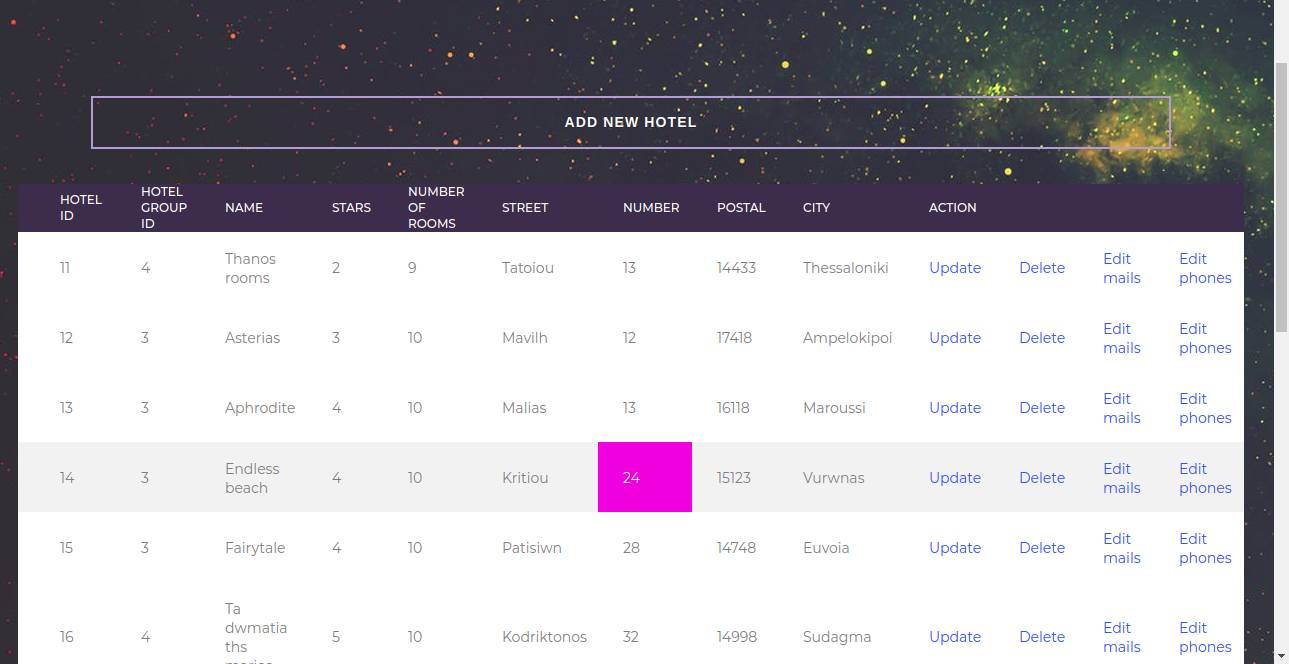
\includegraphics[width=0.9\textwidth]{hoteltables.jpg}
\bigbreak
Επιπλέον, δίπλα σε κάθε εγγραφή δίνεται επιλογή edit\_emails και edit\_phones,όπου μέσω του servlet Hotelmailscontroller και Hotelphonescontroller αντίστοιχα  και δίνοντας τους τις κατάλληλες παραμέτρους και actions ο διαχειριστής μπορεί να δεί σε λίστα τις εγγραφές στους πίνακες hotel\_mails και hotel\_phones, να τις διαγράψει ή να προσθέσει νέες.


\item Rooms. \bigbreak 
Εάν επιλέξει rooms, o διαχειριστής μεταφέρεται στη σελίδα listadminrooms.jsp, όπου του εμφανίζεται ένας πίνακας με όλες τις εγγραφές της σχέσης hotel. Αυτό γίνεται εφικτό μέσω του servlet Hotelscontroller.java δίνoντας του ώς παράμετρο action=listhotelgroups. Δίπλα σε κάθε εγγραφή,υπάρχει η επιλογή να τη διαγράψει ή να την επεξεργαστεί. Επιπλέον,υπάρχει στο πάνω μέρος της οθόνης κουμπί,το οποίο επιλέγει για να προσθέσει νέα εγγραφή. Εάν επιλεγεί να προστεθεί η να ανανεωθεί εγγραφή, ο διαχειριστής μεταφέρεται στη σελίδα adminhotels.jsp, όπου συμπληρώνει τα κατάλληλα πεδία και στη συνέχεια  οι τιμές τους περνάνε ώς παράμετροι στο hotelscontroller και γίνεται αντίστοιχα προσθήκη η ανανέωση στη σχέση hotels. Ομοίως,εάν επιλεγεί διαγραφή πεδίου, το hotel\_id  και το mail/η phone περνάται ώς παράμετρος στο servlet μαζί με action=delete,όπου και πραγματοποιείται η διαγραφή του πεδίου. \bigbreak
Επιπλέον, δίπλα σε κάθε εγγραφή υπάρχει η επιλογή edit\_amenities,η οποία μεταφέρει   τον διαχειριστή στη σελίδα listroomamenities,μέσω του servlet Romamenitiescontroller.java και δίνοντας του ώς παράμετρο το room\_id και action=listamenities.Από τη σελίδα listroomamenities ο διαχειριστής επιλέγωντας add amenity,μεταβαίνει στη σελίδα adminroomamenities,όπου επιλέγει από μια λίστα με amenities ποιες θα προσθέσει.

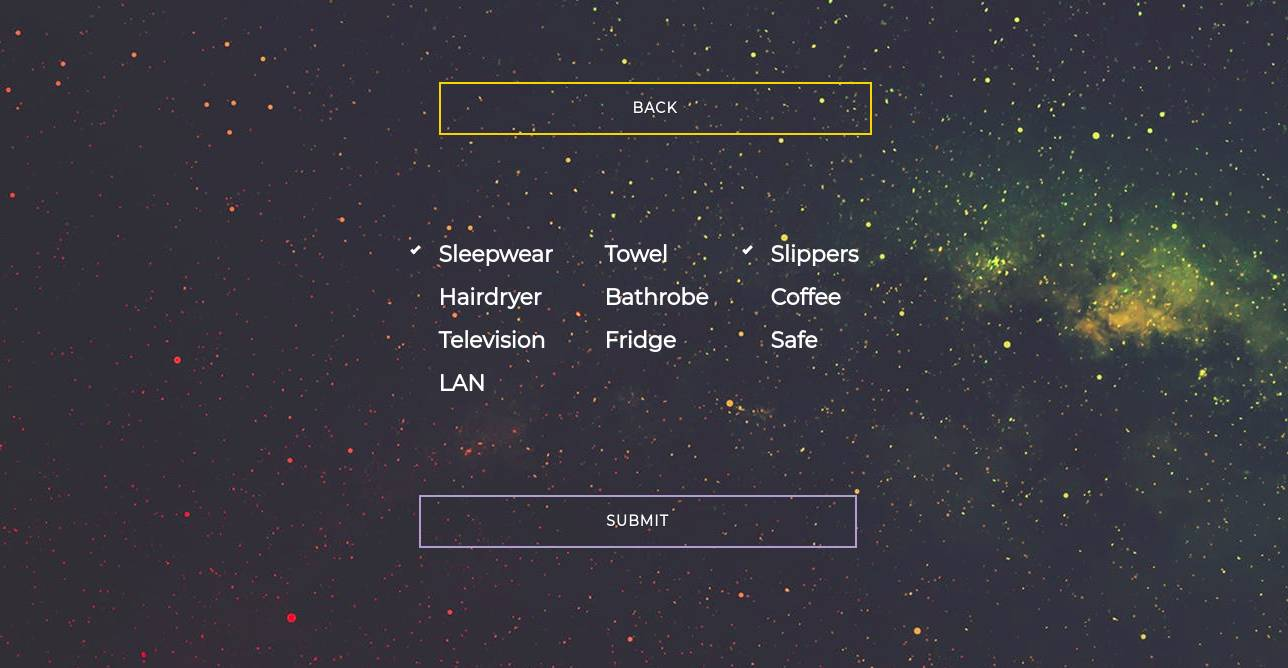
\includegraphics[width=0.9\textwidth]{amenities.jpg}
\bigbreak
\end{itemize}


\end{enumerate}






% TODO add images here.
\section{Σχεσιακό Διάγραμμα}
Το σχεσιακό διάγραμμα της εφαρμογής μας φαίνεται στο ακόλουθο σχήμα:
\begin{figure}[H]
\center
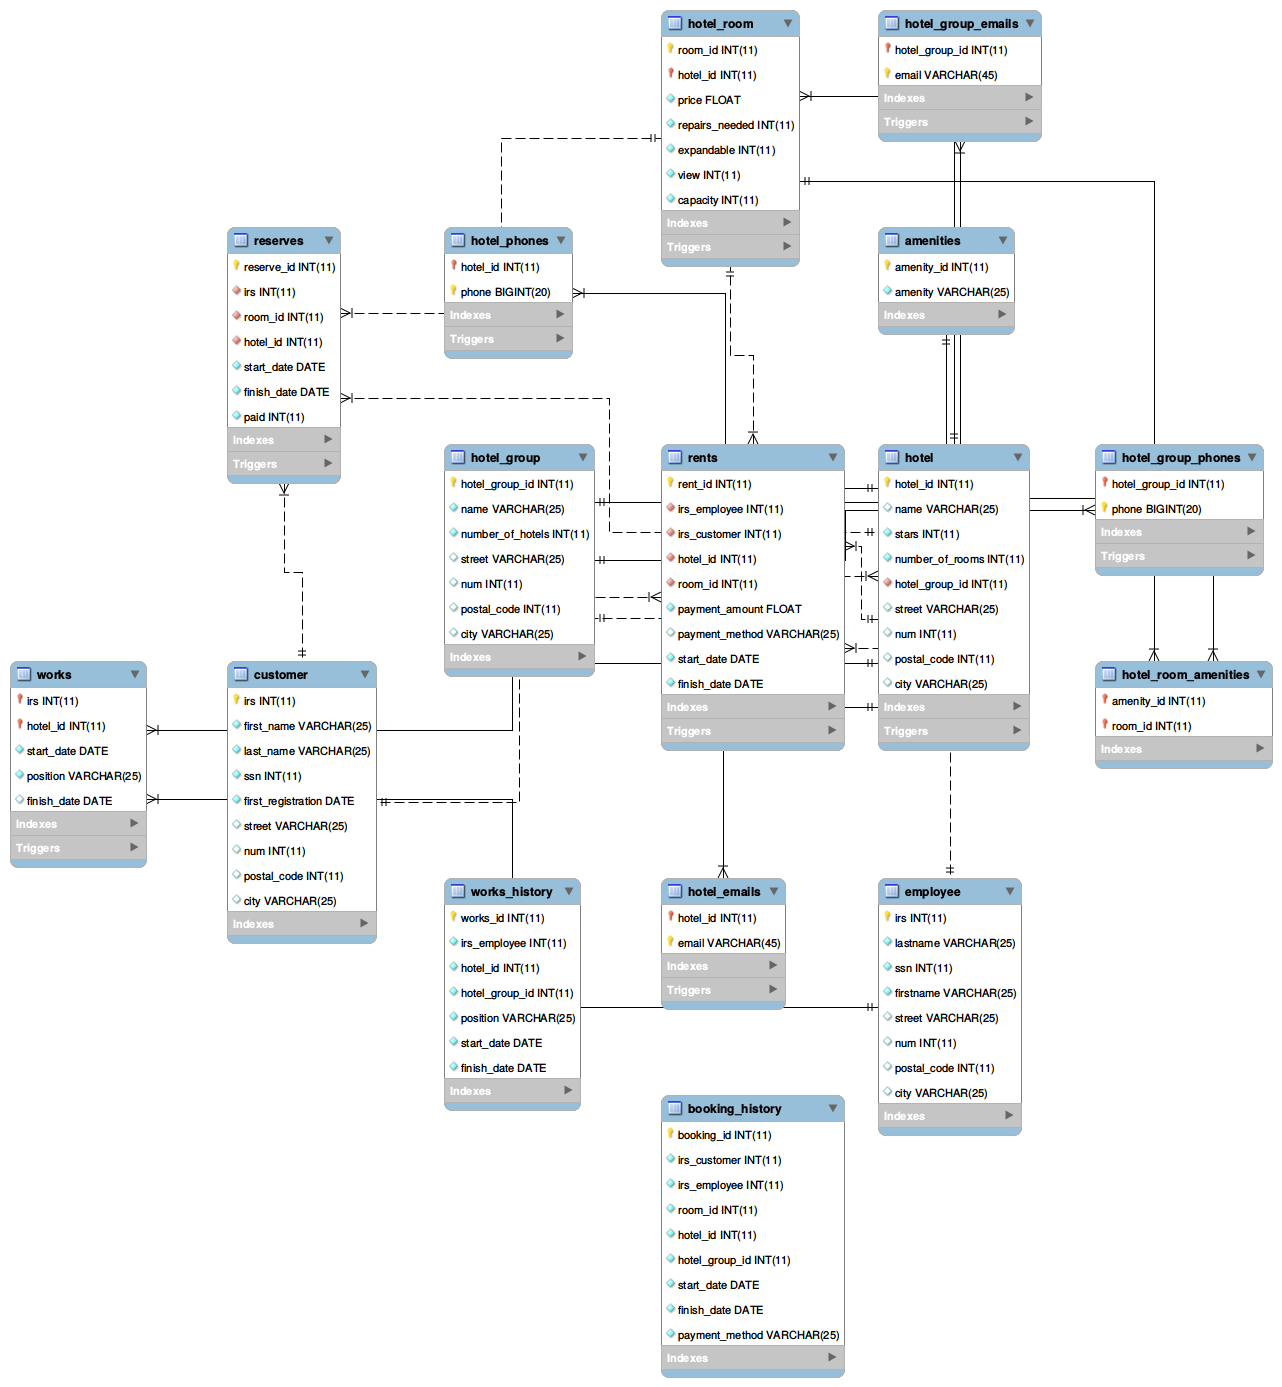
\includegraphics[width=0.9\textwidth]{eer.png}
\bigbreak 
\end{figure}
\underline{Σημείωση: } Το relational model της βάσης μας κατασκευάστηκε από το tables-creator με Reverse Engineering μέσω του εργαλείου mysql-workbench το οποίο εγκαταστήσαμε σε περιβάλλον Ubuntu Linux. Συγκεκριμένα, συνδέουμε τη βάση που κατασκευάσαμε μέσω του tables-creator στο mysql-workbench και στη συνέχεια μέσω των επιλογών Database < Reverse Engineering παράγεται το ζητούμενο διάγραμμα από το mysql-workbench.

\section{Αναλυτική επεξήγηση βάσης και επιλογών σχεδιάσης}

\subsection{Customer}
O πίνακας customer έχει τις εξής στήλες:
\begin{itemize}
\item irs: int \textbf{primary key}. Όπως και στους employee, το irs προσδιορίζει μοναδικά κάθε άνθρωπο άρα και κάθε customer. Συνεπώς, επιλέγεται ως primary key.
\item first\_name: varchar(25).
\item last\_name: varchar(25).
\item ssn: int.
\item first\_registration: date.
\item street: varchar(25).
\item num: int.
\item postal\_code: int.
\item city: varchar(25).
\end{itemize}
\subsection{Hotel Groups}
Ο πίνακας hotel\_group έχει τις ακόλουθες στήλες:
\begin{itemize}
\item hotel\_group\_id: int \textbf{primary key}. Κάθε hotel group προσδιορίζεται μοναδικά από το id του. Προκειμένου να εξασφαλίσουμε τη μοναδικότητα του id ως primary key το βάζουμε \textbf{autoincrement} πεδίο στη βάση.
\item name: varchar(25). Επιλέγουμε να \textbf{προσθέσουμε} τη στήλη name προκειμένου να μην απαιτούνται γνώσεις/πρόσβαση στη βάση προκειμένου ο χρήστης να επιλέξει την αλυσίδα ξενοδοχείων που τον ενδιαφέρει για τις διακοπές του.
\item number\_of\_hotels: int. Η τιμή του πεδίου αυτού \textbf{μεταβάλλεται από triggers}. Παραπέμπουμε στην αντίστοιχη ενότητα για περαιτέρω πληροφορίες.
\item street: varchar(25).
\item num: int.
\item postal\_code: int.
\item city: varchar(25).
\end{itemize}



\subsection{Hotel Group Emails}
Επειδή κάθε hotel group μπορεί να έχει πολλά emails (πλειότιμο) ορίζουμε πίνακα hotel\_group\_emails με \textbf{complex primary key} που αποτελείται από το email και το hotel\_group\_id. Ο πίνακας έχει τις ακόλουθες στήλες:
\begin{itemize}
\item hotel\_id: int \textbf{foreign key} από τον πίνακα hotel\_group.
\item email: varchar(255). Η τιμή του πεδίου αυτού \textbf{ελέγχεται από triggers}.
\end{itemize}


\subsection{Hotel Group Phones}
Επειδή κάθε hotel group μπορεί να έχει πολλά phones (πλειότιμο) ορίζουμε πίνακα hotel\_group\_phones με \textbf{complex primary key} που αποτελείται από το phone και το hotel\_group\_id. Ο πίνακας έχει τις ακόλουθες στήλες:
\begin{itemize}
\item hotel\_id: int \textbf{foreign key} από τον πίνακα hotel\_group.
\item phone: bigint. Η τιμή του πεδίου αυτού \textbf{ελέγχεται από triggers}.
\end{itemize}
\subsection{Hotels}
Ο πίνακας hotel έχει τις ακόλουθες στήλες:
\begin{itemize}
\item hotel\_id: int primary key. Κάθε hotel προσδιορίζεται μοναδικά από το id του. Προκειμένου να εξασφαλίσουμε τη μοναδικότητα του id ως primary key το βάζουμε \textbf{autoincrement} πεδίο στη βάση.
\item name: varchar(25). 
\item stars: int. Το εύρος τιμών ($[1,5]$) αυτού του πεδίου \textbf{ελέγχεται από triggers}. Παραπέμπουμε στη σχετική ενότητα για περισσότερες πληροφορίες.
\item number\_of\_rooms int: Η τιμή του πεδίου αυτού \textbf{μεταβάλλεται από triggers}. Παραπέμπουμε στην αντίστοιχη ενότητα για περαιτέρω πληροφορίες.
\item hotel\_group\_id: int \textbf{foreign key}. Κάθε hotel που εισάγεται στη βάση πρέπει να ανήκει σε κάποιο hotel group. Συνεπώς, το πεδίο hotel\_group\_id ορίζεται ως foreign key από τον πίνακα hotel\_group.
\item street: varchar(25).
\item num: int.
\item postal\_code: int.
\item city: varchar(25).
\end{itemize}

\subsection{Hotel Emails}
Επειδή κάθε hotel μπορεί να έχει πολλά emails (πλειότιμο) ορίζουμε πίνακα hotel\_emails με \textbf{complex primary key} που αποτελείται από το email και το hotel\_id. Ο πίνακας έχει τις ακόλουθες στήλες:
\begin{itemize}
\item hotel\_id: int \textbf{foreign key} από τον πίνακα hotel.
\item email: varchar(255). Η τιμή του πεδίου αυτού \textbf{ελέγχεται από triggers}.
\end{itemize}

\subsection{Hotel Phones}
Επειδή κάθε hotel μπορεί να έχει πολλά phones (πλειότιμο) ορίζουμε πίνακα hotel\_phones με \textbf{complex primary key} που αποτελείται από το phone και το hotel\_id. Ο πίνακας έχει τις ακόλουθες στήλες:
\begin{itemize}
\item hotel\_id: int \textbf{foreign key} από τον πίνακα hotel.
\item phone bigint. Η τιμή του πεδίου αυτού \textbf{ελέγχεται από triggers}.
\end{itemize}


\subsection{Πίνακας employee}
Ο πίνακας employee έχει τις εξής στήλες:
\begin{itemize}
\item irs: int \textbf{primary key}. Όπως φαίνεται από το ER Model κάθε employee προσδιορίζεται μοναδικά από το irs του και συνεπώς επιλέγεται ως primary key. Το irs θεωρούμε ότι είναι ακέραιος αριθμός. 
\item lastname: varchar(25).
\item firstname: varchar(25).
\item ssn: int.
\item street: varchar(25).
\item num: int.
\item postal\_code: int.
\item city: varchar(25).
\end{itemize}

\subsection{Πίνακας works}
Επιλέγουμε να κάνουμε τη σχέση works πίνακα επειδή ένας employee μπορεί να δουλεύει σε πολλά ξενοδοχεία και ένα ξενοδοχείο μπορεί να έχει πολλούς υπαλλήλους. Ο πίνακας works έχει \textbf{complex primary key} που αποτελείται από το \textbf{irs} που προσδιορίζει τον employee και το \textbf{hotel\_id} που προσδιορίζει το ξενοδοχείο.
Οι στήλες του πίνακα είναι:
\begin{itemize}
\item irs: int \textbf{foreign key} από τον πίνακα employee.
\item hotel\_id: int \textbf{foreing key} από τον πίνακα hotel.
\item start\_date: date
\item finish\_date: date
\item position: varchar(25). Για τον πίνακα works \textbf{η στήλη position ελέγχεται από triggers}. Παραπέμπουμε στην αντίστοιχη ενότητα για περισσότερες πληροφορίες.
\end{itemize}
\subsection{Hotel rooms}
Ο πίνακας hotel\_room έχει \textbf{complex} primary key που αποτελείται από τις στήλες \\textbf{room\_id και hotel\_id}. Ο λόγος που επιλέγεται να μπει και το hotel\_id στο primary key είναι νοηματικός: Το hotel\_room είναι weak entity στο ER model και συνεπώς κάθε του entry πρέπει να προσδιορίζεται από τη σχέση που έχει με άλλο πίνακα στη βάση.
\begin{itemize}
\item room\_id: int. Δεδομένου ότι το πεδίο αυτό είναι μέρος του primary key και το άλλο μέρος του primary key μπορεί να είναι κοινό για διαφορετικά entries, το πεδίο αυτό ορίζεται\textbf{ autoincrement}.
\item hotel\_id: int \textbf{foreign key} από τον πίνακα hotel.
\item price: double.
\item repairs\_needed: int. Το εύρος τιμών $[0,1]$ του πεδίου αυτού \textbf{ελέγχεται από triggers}. Παραπέμπουμε στη σχετική ενότητα για περισσότερες πληροφορίες.
\item expandable: int. Το εύρος τιμών $[0,1]$ του πεδίου αυτού \textbf{ελέγχεται από triggers}. Παραπέμπουμε στη σχετική ενότητα για περισσότερες πληροφορίες.
\item view: int.Το εύρος τιμών $[0,1]$ του πεδίου αυτού \textbf{ελέγχεται από triggers}. Παραπέμπουμε στη σχετική ενότητα για περισσότερες πληροφορίες.
\item capacity: int.Το εύρος τιμών $[1,5]$ του πεδίου αυτού \textbf{ελέγχεται από triggers}. Παραπέμπουμε στη σχετική ενότητα για περισσότερες πληροφορίες.
\end{itemize}




\subsection{Πίνακας reserves}
Ο πίνακας reserves περιέχει τις κρατήσεις για τα ξενοδοχεία \textbf{που υπάρχουν ακόμη στη βάση}. Περιέχει τις ακόλουθες στήλες:

\begin{itemize}
\item reserve\_id: int \textbf{primary key autoincrement}. Εξασφαλίζει τη μοναδικότητα κάθε κράτησης.
\item irs: int \textbf{foreign key} από τον πίνακα customer.
\item room\_id: int \textbf{foreign key} από τον πίνακα hotel\_room.
\item hotel\_id: int \textbf{foreign key} από τον πίνακα hotel.
\item hotel\_group\_id: int \textbf{foreign key} από τον πίνακα hotel\_group.
\item start\_date: date.
\item finish\_date: date.
\end{itemize}

\subsection{Πίνακας rents}
Ο πίνακας rents περιέχει τις κρατήσεις για τα ξενοδοχεία \textbf{που υπάρχουν ακόμη στη βάση}. Περιέχει τις ακόλουθες στήλες:
\begin{itemize}
\item rent\_id: int \textbf{primary key autoincrement}. Εξασφαλίζει τη μοναδικότητα κάθε ενοικίασης.
\item irs\_employee: int \textbf{foreign key} από τον πίνακα employee.
\item irs\_customer: int \textbf{foreign key} από τον πίνακα customer.
\item hotel\_id: int \textbf{foreign key} από τον πίνακα hotel.
\item room\_id: int \textbf{foreign key} από τον πίνακα hotel\_room.
\item payment\_amount: float.
\item payment\_method: varchar(25).
\item start\_date: date.
\item finish\_date: date.
\end{itemize}

\subsection{Amenities}
Θεωρήσαμε ότι η καλύτερη σχεδιαστική επιλογή είναι να υπάρχει ένα σύνολο από πιθανά amenities ώστε να υπάρχει ομοιομορφία στην παρεχόμενη πληροφορία των ξενοδοχείων. Έτσι, για τα amenities ορίζουμε δύο πίνακες: amenities, hotel\_room\_amenities.

\subsubsection{Πίνακας amenities}
Ο πίνακας αυτός περιέχει τις ακόλουθες στήλες:
\begin{itemize}
\item amenity\_id: int \textbf{primary key autoincrement}. Είναι το αναγνωριστικό του συγκεκριμένου amenity.
\item amenity: varchar(25). 
\end{itemize}
\subsubsection{Πίνακας hotel\_room\_amenities}
Ο πίνακας αυτός περιέχει την πληροφορία των amenities που έχει κάθε δωμάτιο. Συγκεκριμένα, έχει ένα \textbf{complex primary key} που αποτελείται από το room\_id και το amenity\_id. Οι στήλες του πίνακα είναι τα μέρη του complex primary key του και είναι και οι δύο τύπου int.
\subsection{Επιπλέον πίνακες}
Επειδή πιθανώς χρειαζόμαστε να κρατάμε ένα ιστορικό των ανθρώπων που δούλεψαν στα ξενοδοχεία καθώς και όλες τις ενοικιάσεις-κρατήσεις που έγιναν ακόμα και αν δεν υπάρχει πλέον το δωμάτιο ορίζουμε τους ακόλουθους δύο πίνακες που οι εισαγωγές δεδομένων σε αυτούς γίνονται από triggers: 

\subsubsection{Πίνακας works\_history}
Οι στήλες του πίνακα είναι: 
\begin{itemize}
\item works\_id: int \textbf{primary key autoincrement}. Εξασφαλίζει τη μοναδικότητα κάθε γραμμής.
\item irs\_employee: int 
\item hotel\_id: int 
\item hotel\_group\_id: int
\item position: varchar(25)
\item start\_date: date.
\item finish\_date: date.
\end{itemize}
\subsubsection{Πίνακας booking\_history}
Έχει τις ακόλουθες στήλες:
\begin{itemize}
\item booking\_id: int \textbf{primary key autoincrement}. Εξασφαλίζει τη μοναδικότητα κάθε γραμμής.
\item irs\_customer: int.
\item irs\_employee: int. 
\item room\_id: int.
\item hotel\_id: int.
\item hotel\_group\_id: int.
\item start\_date: date.
\item finish\_date: date.
\item payment\_method: varchar(25).
\end{itemize}

\section{Triggers}
Στην ενότητα αυτοί αναλύουμε όλους τους triggers που έχουμε ορίσει στη βάση δεδομένων μας και βρίσκονται στο αρχείο ./database-setup/database-triggers.sql . \bigbreak 
Οι triggers αυτοί χωρίζονται στις εξής κατηγορίες:
\begin{enumerate}
\item Triggers ελέγχου τιμών
\item Triggers update τιμών
\item Triggers ελέγχου νομιμότητας ενεργειών
\item Triggers διατήρησης ιστορικού
\end{enumerate}

\subsection{Triggers ελέγχου τιμών}
Οι triggers αυτοί ουσιαστικά υλοποιούν τη συνάρτηση check που υπάρχει σε άλλα mysql συστήματα ώστε να διασφαλίσουν ότι μπαίνουν νοηματικά ορθές τιμές. Έχουμε τους ακόλουθους:
\begin{enumerate}
\item check\_for\_hotel\_group\_email\_validity1: Ο trigger αυτός τεστάρει το email που πάει να εισαχθεί σε ένα hotel group απέναντι σε ένα regex expression που ελέγχει την ορθότητα του. Αν δεν περάσει το test, πετάει ένα exception.


\item check\_for\_hotel\_group\_email\_validity2: Ο trigger αυτός τεστάρει το email που πάει να γίνει update σε ένα hotel group απέναντι σε ένα regex expression που ελέγχει την ορθότητα του. Αν δεν περάσει το test, πετάει ένα exception.

\item check\_for\_hotel\_email\_validity1: Ο trigger αυτός τεστάρει το email που πάει να εισαχθεί σε ένα hotel απέναντι σε ένα regex expression που ελέγχει την ορθότητα του. Αν δεν περάσει το test, πετάει ένα exception.

\item check\_for\_hotel\_email\_validity2: Ο trigger αυτός τεστάρει το email που πάει να γίνει update ένα hotel απέναντι σε ένα regex expression που ελέγχει την ορθότητα του. Αν δεν περάσει το test, πετάει ένα exception.

\item check\_for\_hotel\_group\_phone\_validity1: Ο trigger αυτός ελέγχει αν το phone που πάει να εισαχθεί σε ένα hotel\_group είναι έγκυρος αριθμός (\textit{δηλαδή, αν έχει έγκυρο αριθμό ψηφίων}).


\item check\_for\_hotel\_group\_phone\_validity2: Ο trigger αυτός ελέγχει αν το phone που πάει να γίνει update σε ένα hotel\_group είναι έγκυρος αριθμός (\textit{δηλαδή, αν έχει έγκυρο αριθμό ψηφίων}).



\item check\_for\_hotel\_phone\_validity2: Ο trigger αυτός ελέγχει αν το phone που πάει να γίνει εισαχθεί σε ένα hotel είναι έγκυρος αριθμός (\textit{δηλαδή, αν έχει έγκυρο αριθμό ψηφίων}).

\item check\_for\_hotel\_phone\_validity2: Ο trigger αυτός ελέγχει αν το phone που πάει να γίνει update σε ένα hotel group είναι έγκυρος αριθμός (\textit{δηλαδή, αν έχει έγκυρο αριθμό ψηφίων}).


\item check\_for\_stars\_validity1: Ο trigger αυτός αποτρέπει την εισαγωγή ενός ξενοδοχείου αν ο αριθμός των αστεριών του είναι εκτός από τα επιτρεπτά όρια του διαστήματος $[1,5]$.

\item check\_for\_stars\_validity2: Ο trigger αυτός αποτρέπει την αλλαγή των αστεριών ενός ξενοδοχείου αν ο νέος αριθμός είναι εκτός από τα επιτρεπτά όρια του διαστήματος $[1,5]$.

\item check\_for\_hotel\_room\_validity1: Ο trigger αυτός ελέγχει ότι το δωμάτιο που εισάγεται έχει capacity εντός του διαστήματος $[1,5]$ και τις μεταβλητές view, expandable, repairs\_needed εντός του διαστήματος $[0,1]$. Σε διαφορετική περίπτωση, πετάει ένα sql exception.


\item check\_for\_hotel\_room\_validity2: Ο trigger αυτός ελέγχει ότι το δωμάτιο του οποίου ανανεώνονται οι πληροφορίες (update) θα έχει μετά την ανανέωση capacity εντός του διαστήματος $[1,5]$ και τις μεταβλητές view, expandable, repairs\_needed εντός του διαστήματος $[0,1]$. Σε διαφορετική περίπτωση, πετάει ένα sql exception.

\item check\_for\_reserves\_validity1: Ο trigger αυτός ελέγχει ότι το νέο entry που εισάγεται στον πίνακα reserves έχει ορθές νοηματικά τιμές, δηλαδή boolean paid και ημέρα ολοκλήρωσης της κράτησης μεταγενέστερη χρονικά από την ημέρα έναρξης της κράτησης.



\item check\_for\_reserves\_validity2: Ο trigger αυτός ελέγχει ότι το entry που γίνεται update στον πίνακα reserves έχει ορθές νοηματικά τιμές, δηλαδή boolean paid και ημέρα ολοκλήρωσης της κράτησης μεταγενέστερη χρονικά από την ημέρα έναρξης της κράτησης.

\item check\_for\_rent\_validity1: Ο trigger αυτός ελέγχει ότι το νέο entry που εισάγεται στον πίνακα rents έχει ορθές νοηματικά τιμές, δηλαδή μη αρνητικό ποσό πληρωμής και ημέρα ολοκλήρωσης της ενοικίασης μεταγενέστερη χρονικά από την ημέρα έναρξης της ενοικιασης.


\item check\_for\_rent\_validity2: Ο trigger αυτός ελέγχει ότι το entry που γίνεται update στον πίνακα rents έχει ορθές νοηματικά τιμές, δηλαδή μη αρνητικό ποσό πληρωμής και ημέρα ολοκλήρωσης της ενοικίασης μεταγενέστερη χρονικά από την ημέρα έναρξης της ενοικιασης.


\item check\_for\_works\_validity1: Ο trigger αυτός ελέγχει ότι ένας νέος υπάλληλος σε ένα ξενοδοχείο θα έχει ημέρα ολοκλήρωσης συμβολαίου μεταγενέστερη χρονικά από την ημέρα έναρξης συμβολαίου.

\item check\_for\_works\_validity2: Ο trigger αυτός ελέγχει ότι υπάλληλος που γίνεται update σε ένα ξενοδοχείο θα έχει ημέρα ολοκλήρωσης συμβολαίου μεταγενέστερη χρονικά από την ημέρα έναρξης συμβολαίου.


\end{enumerate}

\subsection{Triggers update τιμών}
Σε αυτή την ενότητα βάζουμε όλους τους triggers που πυροδοτούνται για να ανανεώσουν κάποια πληροφορία σε έναν πίνακα όταν σε κάποιον άλλο πίνακα συμβαίνει μια αλλαγή (insert, delete or update). \bigbreak

Συγκεκριμένα, έχουμε τους ακόλουθους triggers:
\begin{enumerate}
\item check\_norooms1: Ο trigger αυτός πυροδοτείται όταν εισάγεται ένα καινούργιο δωμάτιο ώστε ο αριθμός των δωματίων του αντίστοιχου ξενοδοχείου να αυξηθεί.

\item check\_norooms2: Ο trigger αυτός πυροδοτείται όταν διαγράφεται ένα δωμάτιο ώστε ο αριθμός των δωματίων του αντίστοιχου ξενοδοχείου να μειωθεί.

\item check\_nohotels1: O trigger αυτός πυροδοτείται όταν εισάγεται ένα καινούργιο ξενοδοχείο ώστε ο αριθμός των ξενοδοχείων του αντίστοιχου hotel group να αυξηθεί.

\item check\_nohotels2: O trigger αυτός πυροδοτείται όταν διαγράφεται ένα ξενοδοχείο ώστε ο αριθμός των ξενοδοχείων του αντίστοιχου hotel group να μειωθεί.

\item check\_updateroom: Ο trigger αυτός αναλαμβάνει να αλλάξει τους αριθμούς των δωματίων δύο ξενοδοχείων όταν ένα δωμάτιο μεταφέρεται από το ένα ξενοδοχείο στο άλλο.

\item check\_updatehotel: Ο trigger αυτός αναλαμβάνει να αλλάξει τους αριθμούς ξενοδοχείων δύο ξενοδοχειακών αλυσίδων όταν ένα ξενοδοχείο μεταφέρεται από τη μία αλυσίδα στην άλλη.

\item check\_payment: Ο trigger αυτός αναλαμβάνει να θέσει το πεδίο paid του πίνακα reserves στην τιμή 1 όταν γίνεται ενοικίαση για τη συγκεκριμένη κράτηση.

\end{enumerate}

\subsection{Triggers ελέγχου νομιμότητας ενεργειών}
\begin{enumerate}
\item check\_reservation: O trigger αυτός πριν γίνει insert στον πίνακα reserves ελέγχει ότι η κράτηση που πάει να γίνει δεν έχει επικάλυψη με κάποια άλλη κράτηση για το συγκεκριμένο δωμάτιο. Αν υπάρχει επικάλυψη, πετάει exception και αποτρέπει την εισαγωγή.
\item check\_for\_manager\_on\_update: Ο trigger αυτός κάθε φορά που πάει να γίνει update το position ενός εργαζομένου ελέγχει αν μετά το update θα υπάρχει τουλάχιστον ένας manager στο συγκεκριμένο ξενοδοχείο. Σε διαφορετική περίπτωση, πετάει exception και εμποδίζει το update.

\item check\_for\_manager\_on\_delete: Ο trigger αυτός κάθε φορά που πάει να γίνει delete ένας εργαζόμενος ελέγχει αν μετά το delete θα υπάρχει τουλάχιστον ένας manager στο συγκεκριμένο ξενοδοχείο. Σε διαφορετική περίπτωση, πετάει exception και εμποδίζει το delete.


\end{enumerate}

\subsection{Triggers διατήρησης ιστορικού}

\begin{enumerate}
\item create\_workhistory\_entry1: O trigger αυτός για κάθε εισαγωγή στον πίνακα works βάζει τις κατάλληλες πληροφορίες στον πίνακα works\_history προκειμένου να υπάρχει ένα ιστορικό υπαλλήλων στα διάφορα positions για όλα τα ξενοδοχεία και τις ξενοδοχειακές αλυσίδες.

\item create\_workhistory\_entry2: Ο trigger αυτός για κάθε update στον πίνακα works κάνει insert τις κατάλληλες πληροφορίες στον πίνακα works\_history προκειμένου να υπάρχει ένα ιστορικό υπαλλήλων στα διάφορα positions για όλα τα ξενοδοχεία και τις ξενοδοχειακές αλυσίδες.

\item create\_bookinghistory\_entry1: Ο trigger αυτός για κάθε εισαγωγή στον πίνακα rents βάζει τις κατάλληλες πληροφορίες στον πίνακα booking\_history προκειμένου να υπάρχει ένα ιστορικό όλων των κρατήσεων/ενοικιάσεων που έγιναν μέσω της εφαρμογής ακόμα και αν το δωμάτιο, το ξενοδοχείο ή η ξενοδοχειακή αλυσίδα δεν είναι πλέον διαθέσιμα στη βάση.

\item create\_bookinghistory\_entry2: Ο trigger αυτός για κάθε update στον πίνακα rents κάνει το αντίστοιχο update στον πίνακα booking\_history προκειμένου να υπάρχει ένα ιστορικό όλων των κρατήσεων/ενοικιάσεων που έγιναν μέσω της εφαρμογής ακόμα και αν το δωμάτιο, το ξενοδοχείο ή η ξενοδοχειακή αλυσίδα δεν είναι πλέον διαθέσιμα στη βάση.
\end{enumerate}

\subsection{Κώδικας για τους triggers}
Ο κώδικας για τους triggers που αναλύσαμε βρίσκεται στο αρχείο ./database-setup/database-triggers.sql και φαίνεται παρακάτω:

\begin{lstlisting}[language=SQL]
use ntua_db;

delimiter |
create trigger check_norooms1 after insert on hotel_room
	for each row
	begin
	 update hotel set number_of_rooms = number_of_rooms+1 where hotel_id=new.hotel_id;
	end;
|

create trigger check_norooms2 after delete on hotel_room
	for each row
	begin
	 update hotel set number_of_rooms = number_of_rooms-1 where hotel_id=old.hotel_id;
	end;
|

create trigger check_nohotels1 after insert on hotel
	for each row
	begin
	 update hotel_group set number_of_hotels = number_of_hotels+1 where hotel_group_id=new.hotel_group_id;
	end;
|

create trigger check_nohotels2 after delete on hotel
	for each row
	begin
	 update hotel_group set number_of_hotels = number_of_hotels-1 where hotel_group_id=old.hotel_group_id;
	end;
|

create trigger check_updateroom after update on hotel_room
	for each row
	begin
		if (new.hotel_id <> old.hotel_id) then
		 update hotel set number_of_rooms=number_of_rooms+1 where hotel_id=new.hotel_id;
		 update hotel set number_of_rooms=number_of_rooms-1 where hotel_id=old.hotel_id;
		end if;
	end;

|

create trigger check_updatehotel after update on hotel
	for each row
	begin
		if (new.hotel_group_id <> old.hotel_group_id) then
		
	 	 update hotel_group set number_of_hotels=number_of_hotels+1 where hotel_group_id=new.hotel_group_id;
	 	 update hotel_group set number_of_hotels=number_of_hotels-1 where hotel_group_id=old.hotel_group_id;
	 	
	 	end if;
	end;
|

create trigger check_payment after insert on rents
	for each row
	begin
		update reserves set paid=1 where (irs=new.irs_customer and room_id=new.room_id and start_date=new.start_date and finish_date=new.finish_date);
	end;
|

create trigger check_reservation before insert on reserves
	for each row
	begin
		if (exists(select * from reserves where new.room_id=room_id and not(new.finish_date<=start_date or new.start_date>=finish_date))) then
		 signal sqlstate '45000' set message_text = 'Sorry,another user booked the room';
		end if;
	end;

|

create trigger check_for_hotel_group_email_validity1 before insert on hotel_group_emails
	for each row
	begin
		if (new.email not like '%@%.%' or new.email like '@%' or new.email like '%@%@%' ) then
			signal sqlstate '45000' set message_text = 'Wrong email';
		end if;
	end;
|

create trigger check_for_hotel_group_email_validity2 before update on hotel_group_emails
	for each row
	begin
		if (new.email not like '%@%.%' or new.email like '@%' or new.email like '%@%@%' ) then
			signal sqlstate '45000' set message_text = 'Wrong email';
		end if;
	end;
|


create trigger check_for_hotel_email_validity1 before insert on hotel_emails
	for each row
	begin
		if (new.email not like '%@%.%' or new.email like '@%' or new.email like '%@%@%' ) then
			signal sqlstate '45000' set message_text = 'Wrong email';
		end if;
	end;
|

create trigger check_for_hotel_email_validity2 before update on hotel_emails
	for each row
	begin
		if (new.email not like '%@%.%' or new.email like '@%' or new.email like '%@%@%' ) then
			signal sqlstate '45000' set message_text = 'Wrong email';
		end if;
	end;
|

create trigger check_for_hotel_group_phone_validity1 before insert on hotel_group_phones
	for each row
	begin
		if (new.phone<10000000 or new.phone>999999999999) then
			signal sqlstate '45000' set message_text = 'Wrong phone';
		end if;
	end;
|

create trigger check_for_hotel_group_phone_validity2 before update on hotel_group_phones
	for each row
	begin
		if (new.phone<10000000 or new.phone>999999999999) then
			signal sqlstate '45000' set message_text = 'Wrong phone';
		end if;
	end;
|

create trigger check_for_hotel_phone_validity1 before insert on hotel_phones
	for each row
	begin
		if (new.phone<10000000 or new.phone>999999999999) then
			signal sqlstate '45000' set message_text = 'Wrong phone';
		end if;
	end;
|

create trigger check_for_hotel_phone_validity2 before update on hotel_phones
	for each row
	begin
		if (new.phone<10000000 or new.phone>999999999999) then
			signal sqlstate '45000' set message_text = 'Wrong phone';
		end if;
	end;
|


create trigger check_for_stars_validity1 before insert on hotel
	for each row
	begin
		if (new.stars<=0 or new.stars>5) then
			signal sqlstate '45000' set message_text = 'Wrong star argument';
		end if;

	end;
|

create trigger check_for_stars_validity2 before update on hotel
	for each row
	begin
		if(new.stars<=0 or new.stars>5) then
			signal sqlstate '45000' set message_text = 'Wrong star argument';
		end if;
	end;
|
			 

create trigger check_for_hotel_room_validity1 before insert on hotel_room
	for each row
	begin
		if (new.view<0 or new.view>1 or new.capacity>4 or new.capacity<0 or new.expandable<0 or new.expandable>1 or new.price<0) then
			signal sqlstate '45000' set message_text = 'Wrong hotel room arguments';
		end if;
	end;
|

create trigger check_for_hotel_room_validity2 before update on hotel_room
	for each row
	begin
		if (new.view<0 or new.view>1 or new.capacity>4 or new.capacity<0 or new.expandable<0 or new.expandable>1 or new.price<0) then
			signal sqlstate '45000' set message_text = 'Wrong hotel room arguments';
		end if;
	end;
|

create trigger check_for_reserves_validity1 before insert on reserves
	for each row
	begin
		if (new.paid<0 or new.paid>1 or new.finish_date<=new.start_date) then 
			signal sqlstate '45000' set message_text = 'Wrong reservation';
		end if;
	end;
|


create trigger check_for_reserves_validity2 before update on reserves
	for each row
	begin
		if (new.paid<0 or new.paid>1 or new.finish_date<=new.start_date) then 
			signal sqlstate '45000' set message_text = 'Wrong reservation';
		end if;
	end;
|


create trigger check_for_rent_validity1 before insert on rents
	for each row
	begin
		if (new.payment_amount<0 or new.finish_date <= new.start_date ) then 
			signal sqlstate '45000' set message_text = 'Error in rents arguments';
		end if;
	end;	
|


create trigger check_for_rent_validity2 before update on rents
	for each row
	begin
		if (new.payment_amount<0 or new.finish_date <= new.start_date ) then 
			signal sqlstate '45000' set message_text = 'Error in rents arguments';
		end if;
	end;	
|


create trigger check_for_works_validity1 before insert on works
	for each row
	begin
		if (new.finish_date<new.start_date) then
			signal sqlstate '45000' set message_text = 'Work dates error';
		end if;
	end;
|


create trigger check_for_works_validity2 before update on works
	for each row
	begin
		if (new.finish_date<new.start_date) then
			signal sqlstate '45000' set message_text = 'Work dates error';
		end if;
	end;
|


	
create trigger check_for_manager_on_update before update on works
	for each row 
	begin
		if (new.position <> old.position and old.position='manager') then 
			if ( not exists(select * from works where new.hotel_id=hotel_id and new.position='manager'and new.finish_date>curdate())) then 
				signal sqlstate '45000' set message_text = 'Every hotel must have a manager';
			end if;
		end if;
	end;
|


create trigger check_for_manager_on_delete before delete on works
	for each row 
	begin
		if (old.position='manager') then
			if ( (select count(position) from works where old.position='manager' and old.finish_date>curdate())>1) then 
				signal sqlstate '45000' set message_text = 'Every hotel must have a manager';
			end if;
		end if;
	end;
|

create trigger create_workhistory_entry1 after insert on works
	for each row
	begin
		insert into works_history(irs_employee,hotel_id,hotel_group_id,position,start_date,finish_date) values (new.irs,new.hotel_id,(select hotel_group_id from hotel where hotel_id=new.hotel_id),new.position,new.start_date,new.finish_date);
        end;
|

create trigger create_workhistory_entry2 after update on works
	for each row
	begin
		insert into works_history(irs_employee,hotel_id,hotel_group_id,position,start_date,finish_date) values (new.irs,new.hotel_id,(select hotel_group_id from hotel where hotel_id=new.hotel_id),new.position,new.start_date,new.finish_date);
        end;
|

create trigger create_bookinghistory_entry1 after insert on rents
	for each row
	begin
		insert into booking_history(irs_employee,irs_customer,room_id,hotel_id,hotel_group_id,start_date,finish_date,payment_method) values (new.irs_employee,new.irs_customer,new.room_id,new.hotel_id,(select hotel_group_id from hotel where hotel_id=new.hotel_id),new.start_date,new.finish_date,new.payment_method);
	end;
|

create trigger create_bookinghistory_entry2 after update on rents
	for each row
	begin
		update booking_history set irs_employee=new.irs_employee,irs_customer=new.irs_customer,room_id=new.room_id,start_date=new.start_date,finish_date=new.finish_date,payment_method=new.payment_method,hotel_id=new.hotel_id,hotel_group_id=(select hotel_group_id from hotel where hotel_id=new.hotel_id);
	end;
|
delimiter ;


\end{lstlisting}



\section{Περαιτέρω περιορισμοί}
Στην ενότητα αυτή αναλύουμε περιορισμούς που δεν καλύπτονται από τους triggers και από τις σχεδιαστικές επιλογές που κάναμε. Η ανάλυση γίνεται τόσο σε επίπεδο εφαρμογής όσο και σε επίπεδο βάσης δεδομένων.
\subsection{Επίπεδο βάσης}
Εκτός από τους περιορισμούς που εισάγουν τα triggers έχουμε και τους ακόλουθους περιορισμούς:
\begin{itemize}
\item Όλα τα foreign key constraints έχουν οριστεί με on delete cascade property προκειμένου να επιτρέπονται τα deletes στους πίνακες "γονείς". Αυτό δεν σημαίνει ότι χάνεται χρήσιμη πληροφορία με την διαγραφή ενός ξενοδοχείου ή μιας ξενοδοχειακής αλυσίδας. Διατηρούμε μέσω triggers ενημερωμένους για όλο το ιστορικό τους πίνακες booking\_history και works\_history οι οποίοι δεν έχουν foreign key constraint ώστε να έχουμε όλο το ιστορικό των αλλαγών που αφορά employees και ενοικιάσεις σε δωμάτια.
\item Όλα τα πεδία των πινάκων που αντιστοιχούν σε entities και σχέσεις του ER Model έχουν οριστεί NOT NULL καθώς αφενός θεωρούμε ότι είναι χρήσιμες πληροφορίες που διασφαλίζουν την πληρότητα και την ομοιομορφία της βάσης και αφετέρου έτσι είναι ευκολότερα διαχειρίσμος και επεκτάσιμος ο κώδικας της εφαρμογής.
\item Η σχέση works έχει ως complex primary key το hotel\_id μαζί το irs του υπαλλήλου. Αυτό σημαίνει ότι δεν μπορεί ένας υπάλληλος να δουλέυει στο ίδιο ξενοδοχείο σε δύο positions. Ο περιορισμός αυτός τέθηκε καθώς δεν προκύπτει σενάριο διπλοθεσίας από την εκφώνηση. Σε μια τέτοια εκδοχή, θα έπρεπε να οριστεί ένα autoincrement primary key στον πίνακα works. Στην παρούσα μορφή, ο περιορισμός αυτός όμως διασφαλίζει και ότι υπάρχει μοναδικό record στον πίνακα works για κάθε υπάλληλο ενώ στο σενάριο του autoincrement primary key δεν θα υπήρχε τέτοιος περιορισμός. Σημειώνουμε, ότι το να δουλεύει ένας υπάλληλος σε δύο διακριτά χρονικά διαστήματα στο ίδιο ξενοδοχείο προβλέπεται κανονικά από τη βάση με τη διαγραφή του υπαλλήλου και την επανατοποθέτηση του μετά την επαναπρόσληψη. Η πρώτη πρόσληψη δεν χάνεται καθώς κρατάμε το πλήρες ιστορικό με triggers στον πίνακα works\_history. 
\item Ορίζουμε έναν πίνακα amenities στον οποίο μπαίνουν τα πιθανά amenities, αντί να αφήνουμε στον πίνακα hotel\_room\_amenities να υπάρχει μια στήλη varchar(25) για τα amenities. Αυτή η επιλογή γίνεται καθώς θεωρούμε πως είναι αυθαίρετο κάθε ξενοδοχείο να βάζει με δικό του τρόπο τα amenities (πχ: tv ή television ; ) και αν επιτρέπαμε κάτι τέτοιο θα είχαμε νοηματικά όμοια αντικείμενα να είναι ασυσχέτιστα στη βάση δεδομένων μας.
\end{itemize}
\subsection{Επίπεδο εφαρμογής}
Σε επίπεδο εφαρμογής, έχουμε ορίσει τους ακόλουθους περιορισμούς:
\begin{enumerate}
\item Δεν μπορείς να ψάξεις ξενοδοχείο ή να κάνεις κράτηση για ημερομηνίες που ανήκουν στο παρελθόν (μήνυμα λάθους: \textit{'You can't book the past'}). 
\item Δεν μπορείς να ψάξεις ξενοδοχείο ή να κάνεις κράτηση για start date που είναι μεταγενέστερο χρονικά του finish date (μηνύμα λάθoυς: \textit{'Dates collision'}). 
\item Μπορείς να αναζητήσεις ξενοδοχείο αφήνοντας κενές τις ημερομηνίες έναρξης και λήξης ή συμπληρώνοντας και τις δύο. Αν συμπληρώσεις μόνο τη μία από τις δύο παίρνεις σχετικό μήνυμα λάθους για να αλλάξεις την επιλογή σου.
\item Δεν μπορείς να κάνεις κράτηση αν δεν έχεις ορίσει και το start και το finish date.
\item Οι επιλογές ως προς το payment method στο rent είναι MasterCard, PayPal, Cash καθώς θεωρούμε ότι βάζοντας selectbox στις επιλογές διασφαλίζεται μια ομοιομορφία στη βάση (αντί να αφήνεις για παράδειγμα ελεύθερο κείμενο για εισαγωγή στη φόρμα).
\end{enumerate}





\section{Εφαρμογή και SQL}
Στην ανάπτυξη της εφαρμογής χρησιμοποιήθηκαν διάφορα sql statements για την επικοινωνία, την τροποποίηση και την ανάκτηση δεδομένων από την βάση. Στην ενότητα αυτή, εξηγούμε τον τρόπο λειτουργίας ορισμένων λειτουργιών της εφαρμογής από την σκοπιά της sql.

\subsection{Selections}
Στην υποενότητα αυτή παραθέτουμε μερικά από τα selection queries που γίνονται μέσω της εφαρμογής μας.
\begin{enumerate}
\item Ιδιότητα city από τις εγγραφές της σχέσης hotel, καταργώντας τις διπλές τιμές \bigbreak 
\begin{lstlisting}[language=SQL]
select distinct cities from hotel
\end{lstlisting}
\item Όλες οι εγγραφές στη σχέση hotel\_mails, στις οποίες η ιδιότητα hotel\_id έχει την τιμή 1 \bigbreak
\begin{lstlisting}[language=SQL]
select  *  from hotel_mails where hotel_id=1  ;
\end{lstlisting}
\item hotel\_id από τις εγγραφές στη σχέση works που πληρούν τις προυποθέσεις το ΑΦΜ του υπαλλήλου να είναι 1245 και να είναι ακόμα ενεργός στο συγκεκριμένο ξενοδοχείο. \bigbreak
\begin{lstlisting}[language=SQL]
select hotel_id from works where irs=1245 and finish_date>curdate();
\end{lstlisting}
\end{enumerate}
\subsection{Ενώσεις - Joins}
Στην εφαρμογή μας χρησιμοποιούμε συχνά selection queries που γίνονται σε joined πίνακες. 
Ένα παράδειγμα για την περιγραφή των amenities, που παρέχονται από το δωμάτιο με τον δοσμένο κωδικό δωματίου:
\begin{lstlisting}[language=SQL]
select hotel_room_amenities.room_id,amenities.amenity from hotel_room_amenities inner join amenities on hotel_room_amenities.amenity_id=amenities.amenity_id where room_id=2
\end{lstlisting}

\subsection{Insertions}
Τροποποιήσεις στη βάση γίνονται και με την εισαγωγή νέων στοιχείων. Για παράδειγμα, με το ακόλουθο query Θέτουμε νέες τιμές στις ιδιότητες της εγγραφής του πίνακα hotel, για την οποία το hotel\_id είναι αυτό που ορίστηκε:
\begin{lstlisting}[language=SQL]
update hotel set hotel_group_id=?,name=? ,stars=?, street=?, num=?, postal_code=?, city=? where hotel_id=?;
\end{lstlisting}

\subsection{Deletions}
Ο admin της βάσης από την εφαρμογή μας μπορεί αφού συνδεθεί να διαγράψει στοιχεία από τη βάση. Για παράδειγμα, η διαγραφή ενός ξενοδοχείου μέσω της εφαρμογής μας μπορεί να πυροδοτήσει το ακόλουθο query:
\begin{lstlisting}[language=SQL]
delete from hotel where hotel_id=2;
\end{lstlisting}

\subsection{Δυναμικά queries - Παράδειγμα: αναζήτηση δωματίων με βάση πολλά κριτήρια}
Τα περισσότερα queries στην εφαρμογή μας αναπτύσσονται δυναμικά, με την έννοια ότι ξεκινάμε από ένα μικρό query και το μεγαλώνουμε ανάλογα με το αν ο χρήστης έχει συμπληρώσει ή όχι πεδία της φόρμας. Στην υποενότητα αυτή αναλύουμε το σύνθετο query της αναζήτησης δωματίου με βάση όλα τα κριτήρια που παρέχονται στην εφαρμογή. 
Μελετάμε τη σύνθετη περίπτωση που ο χρήστης έχει επιλέξει και συγκεκριμένο αριθμό δωματίων που αναζητά. 

\bigbreak 
Αρχικά, παραθέτουμε το ακόλουθο κομμάτι κώδικα:
\begin{lstlisting}[language=Java]
String columns="hotel_group.name as name2,hotel.name,room_id, hotel_room.hotel_id, price, repairs_needed, expandable, view, capacity, stars, hotel.hotel_group_id, hotel.street, hotel.num, hotel.postal_code, hotel.city";

String columns2="tmp.name2,tmp.name,tmp.room_id, tmp.hotel_id, price, repairs_needed, expandable, view, capacity, stars, tmp.hotel_group_id, tmp.street, tmp.num, tmp.postal_code, tmp.city";

String firstQuery="create temporary table tmp select "+columns+" from hotel_room inner join hotel on hotel_room.hotel_id=hotel.hotel_id inner join hotel_group on hotel.hotel_group_id=hotel_group.hotel_group_id where (";

 if (! stars.equals("_______")) {
   			 firstQuery=firstQuery+"stars="+stars+" and ";
   		 }
   		 if (! capacity.equals("_______")) {
   			 firstQuery=firstQuery+"capacity >="+capacity+ " and ";
   		 }
   		 if (!group.equals("_______")) {
   			 firstQuery=firstQuery+"hotel_group.hotel_group_id="+group+ " and ";
   		 }
   		 
   		 if (!price.equals("")) {
   			 firstQuery=firstQuery+"hotel_room.price<="+price+" and ";
   		 }

   		 int len=locations.length;
   		 int index=1;
   		 if (len>0) {
   			 firstQuery=firstQuery+"hotel.city in (";
   		 }
   		 for (String x : locations) {
   			 if (index==len) {
   				 firstQuery=firstQuery+"\'"+x+"\'"+") and ";
   			 }
   			 else {
   				 firstQuery=firstQuery+"\'"+x+"\'"+",";
   			 }
   			 index=index+1;
   		 }

\end{lstlisting}

Με αυτόν τον τρόπο, σύμφωνα με το ποια κριτήρια ο πελάτης έχει ορίσει επιστρέφονται σε προσωρινό πίνακα οι ιδιότητες  hotel\_group.name,hotel.name,room\_id, hotel\_room.hotel\_id, price, repairs\_needed, expandable, view, capacity, stars, hotel.hotel\_group\_id, hotel.street, hotel.num, hotel.postal\_code, hotel.city από την ένωση των σχέσεων hotel\_room,hotel και hotel\_group.

Στη συνέχεια με τον εξής κώδικα:
\begin{lstlisting}[language=Java]
String case1="create temporary table tmp2 select distinct "+columns2+" from tmp order by "+option+";";
 String secondQuery="create temporary table tmp2 select distinct "+columns2+" from tmp left join reserves on tmp.room_id=reserves.room_id where ( (reserves.room_id is null) or ("; 

secondQuery=secondQuery+"(finish_date<\'"+start+"\') or (start_date>\'"+finish+"\')";

\end{lstlisting}


Γίνεται ένωση της προηγούμενης προσωρινής σχέσης με τη σχέση  reserve και επιστρέφονται σε δέυτερο προσωρινό πίνακα οι ιδιότητες των δωματίων, τα οποία είναι διαθέσιμα τις ημερομηνίες που εισήγαγε(αν εισήγαγε) ο πελάτης. \bigbreak
Τέλος, έχουμε:
\begin{lstlisting}[language=Java]
String helpQuery="create temporary table tmp3 like tmp2";
helpQuery="insert tmp3 select * from tmp2";

if (!num.equals("")) {
   			 finalQuery="select * from tmp2 where hotel_id in (select hotel_id from tmp3 group by hotel_id having count(hotel_id)>="+num+")";
   		 }
   		 else {
   			 finalQuery="select * from tmp2";
   		 }
\end{lstlisting}


Εδώ δημιουργείται ένα αντίγραφο του δεύτερου προσωρινού πίνακα και εμφανίζονται στο χρήστη οι ιδιότητες των δωματίων, τα οποία πληρούν επιπροσθέτως το κριτήριο το ξενοδοχείο, στο οποίο ανήκουν να έχει διαθέσιμο αριθμό δωματίων ίσο ή μεγαλύτερο με αυτό που έχει επιλέξει ο χρήστης.

\subsection{Δημιουργία views βάσης}

Στην εκφώνηση ζητείται να δημιουργήσουμε views της βάσης στα οποία ο χρήστης θα μπορεί να βλέπει τον αριθμό των διαθέσιμων δωματίων ανά capacity και τον αριθμό των διαθέσιμων δωματίων ανά location. 
Για την δημιουργία των συγκεκριμένων views τρέχουμε τα ακόλουθα queries που βρίσκονται στο φάκελο database-setup στο αρχείο database-views.sql :
\begin{lstlisting}[language=SQL]
create view hotel_room_capacity_view as select capacity,count(room_id) as rooms_per_capacity from hotel_room where room_id not in (select room_id from reserves where curdate() between start_date and finish_date) group by capacity; 
create view hotel_room_location_view as select htl.city,count(htl_room.room_id) as rooms_per_city from hotel as htl inner join hotel_room as htl_room on htl.hotel_id=htl_room.hotel_id where htl_room.room_id not in (select room_id from reserves where curdate() between start_date and finish_date) group by city; 
\end{lstlisting}
Τα views αυτά ο χρήστης μπορεί να τα προσπελάσει από τη σελίδα hotelSelection.jsp πατώντας τα αντίστοιχα buttons.
\section{Ευρετήρια}
Τα ευρετήρια επιβαρύνουν τη διαδικασία των insertions, μπορούν όμως σε ορισμένες περιπτώσεις να επιταχύνουν σημαντικά το selection. Ιδιαίτερα στην περίπτωση που το selection γίνεται συνήθως με κάποιο where clause που αφορά στήλη που δεν είναι key, τα indexes μπορούν να επιταχύνουν σημαντικά την διαδικασία.
\subsection{Ευρετήρια που ορίζει η mysql}
Η mysql ορίζει από μόνη της ως ευρετήρια όλα τα primary και τα foreign keys. Συνεπώς, όλα τα πεδία που έχουμε ορίσει ως primary ή foreign keys υφίστανται indexing. 
\subsection{Δικά μας ευρετήρια}
Η χρήση ευρετηρίων έχει νόημα στις περιπτώσεις που τα selections είναι πολύ περισσότερα από τα insertions και ιδιαίτερα όταν γίνονται με where clause που αφορά στήλες που δεν είναι keys. Αυτή ακριβώς είναι η περίπτωση της αναζήτησης δωματίου: Ψάχνουμε πολύ συχνότερα δωμάτια για ένα προορισμό από ότι πραγματικά κλείνουμε, και όταν ψάχνουμε, ψάχνουμε με βάση τα start και finish dates. Είναι λοιπόν χρήσιμο, στους πίνακες reserves και rents που γίνονται οι αναζητήσεις να χρησιμοποιήσουμε indexes. 
Έτσι, ορίζουμε τα ακόλουθα δύο indexes:
\begin{lstlisting}[language=SQL]
create index reserves_date_index on reserves (start_date, finish_date);
create index rents_date_index on rents (start_date, finish_date);
\end{lstlisting}
Ακόμη, όταν ψάχνουμε στο ιστορικό των εργαζομένων, μας αφορούν συνήθως πληροφορίες όπως πόσοι εργαζόμενοι υπήρχαν σε μια συγκεκιμένη χρονική περίοδο. Η αναζήτηση γίνεται με βάση τα dates και όχι με βάση κάποιο κλειδί. Άρα, έχει και εδώ πιθανώς νόημα να ορίσουμε το index:
\begin{lstlisting}[language=SQL]
create index works_history_date_index on works_history (start_date, finish_date);
\end{lstlisting}
Τέλος, για τα bookings που έχουν γίνει μας ενδιαφέρει συχνά ο τρόπος πληρωμής και οι ημερομηνίες (παρά το booking id). Άρα, ορίζουμε και εδώ το index:
\begin{lstlisting}[language=SQL]
create index booking_history_index on booking_history (start_date,finish_date,payment_method);
\end{lstlisting}
\section{Σύστημα και γλώσσες προγραμματισμού}
\begin{enumerate}
\item Το παρόν project υλοποιήθηκε σε Linux Ubuntu σύστημα. 
\item Για την υλοποίηση της Βάσης Δεδομένων χρησιμοποιείται MySQL Server (έκδοση 5.7.22). \bigbreak 
\item Για το server-side της εφαρμογής χρησιμοποιείται Java.  
\item Για την επικοινωνία μεταξύ client και server χρησιμοποιήθηκε Apache Tomcat.
\item Ως προς το front-end της εφαρμογής χρησιμοποιήθηκε html για την εισαγωγή των στοιχείων της σελίδας, css για τον καλλωπισμό των στοιχείων αυτών και Javascript για form validation, δημιουργία διαδραστικών στοιχείων (όπως κουμπιών), δημιουργία ενός custom calendar, κ.α. . Για το css χρησιμοποιήσαμε το bootstrap framework και ιδιαίτερα ότι αφορά τους containers και το grid σύστημα που προσφέρει για responsive στοίχιση στοιχείων.
\end{enumerate}
Πιο συγκεκριμένα, χρησιμοποιούνται jsp αρχεία τα οποία περιέχουν Java κώδικα και μέσω του Apache Tomcat γίνονται render σε html ώστε να μπορεί να τα βλέπει ο client. Τα αρχεία αυτά επικοινωνούν με τη βάση μέσω κατάλληλων Servlets (Java files) τα οποία συνομιλούν με τη ΒΔ και στέλνουν πληροφορίες πίσω στα jsp files για εμφάνιση στο χρήστη της εφαρμογής.

\section{Αναλυτικά βήματα εγκατάστασης της εφαρμογής}
Τα βήματα που χρειάζεται να υλοποιήσει κάποιος προκειμένου να εγκαταστήσει την εφαρμογή μας σε σύστημα Linux είναι τα ακόλουθα:
\begin{enumerate}

\item Εγκατάσταση mysql. Σε ubuntu, η εγκατάσταση μπορεί να γίνει από το terminal με τη χρήση της εντολής:
\begin{lstlisting}[language=bash]
sudo apt-get install mysql-server
\end{lstlisting}
\item Δημιουργία βάσης δεδομένων. \bigbreak 
Αφού ολοκληρώσουμε με το installation και το setup του mysql-server (ορίζοντας κωδικό για το χρήστη root) πληκτρολογούμε στο terminal:
\begin{lstlisting}[language=bash]
mysql -u root -p
\end{lstlisting}
Αφού εισάγουμε τον κωδικό και συνδεθούμε γράφουμε:
\begin{lstlisting}[language=SQL]
create database ntua_db;
\end{lstlisting}
\item Δημιουργία πινάκων στη βάση δεδομένων. \bigbreak 
Κλείνουμε το session με τη mysql, κάνουμε cd στο φάκελο database-setup και τρέχουμε την ακόλουθη εντολή:
\begin{lstlisting}[language=SQL]
mysql -u root -p ntua_db < tables-creator.sql
\end{lstlisting}
\item Εισαγωγή των triggers. \bigbreak 
Για να εισάγουμε στη βάση δεδομένων μας τους triggers που έχουμε ορίσει γράφουμε:
\begin{lstlisting}[language=SQL]
mysql -u root -p ntua_db < database-triggers.sql
\end{lstlisting}
\item Αρχικοποίηση με δεδομένα. \bigbreak 
Για να αρχικοποιήσουμε τη βάση δεδομένων μας τρέχουμε στο terminal:
\begin{lstlisting}[language=SQL]
mysql -u root -p ntua_db < database-initializer.sql
\end{lstlisting}
\item Δημιουργία views βάσης. \bigbreak 
\begin{lstlisting}[language=SQL]
mysql -u root -p ntua_db < database-views.sql
\end{lstlisting}
\item Εγκατάσταση JAVA. \bigbreak 
\textit{Στο τέλος της εγκατάστασης, θα πρέπει να υπάρχει στο .bashrc ορισμένη η μεταβλητή JAVA\_HOME που να δείχνει στο φάκελο εγκατάστασης της JAVA στον υπολογιστή.}
\item Εγκατάσταση Eclipse.
\item Εγκατάσταση Apache Tomcat. \bigbreak 
\textit{Στο τέλος της εγκατάστασης, θα πρέπει να υπάρχει στο .bashrc ορισμένη η μεταβλητή CATALINA\_HOME που να δείχνει στο φάκελο εγκατάστασης του Apache Tomcat στον υπολογιστή.}
\item Download του binary file του MySQL JDBC Driver.
\item Αποσυμπίεση του τελευταίου αρχείου
\item Μεταφορά του jar file που προέκυψε από την αποσυμπίεση στο φάκελο \$CATALINA\_HOME/lib. \bigbreak
\underline{Σημείωση: } \textit{Η μεταβλητή CATALINA\_HOME} ορίστηκε στο βήμα 9.
\item Import στο Eclipse του project. Αυτό γίνεται ακολουθώντας τη διαδρομή: File > Import
\item Εισαγωγή ενός instance του Apache Tomcat Server στο Eclipse. \bigbreak 
Για να το πετύχουμε αυτό ακολουθούμε τη διαδρομή στο Eclipse: 
Window > Preferences > Server > Runtime Environments > Αdd και διαλέγουμε από τη λίστα τον Apache Tomcat στην έκδοση που τον κατεβάσαμε.
\item Configuration του Apache Tomcat Instance. \bigbreak
Προκειμένου να μπορέσει το Instance με τη βάση δεδομένων μας πρέπει να μπορέσει να τη δει. Για να συμβεί αυτό απαιτείται μια διαδικασία configuration. Συγκεκριμένα, αλλάζουμε το αρχείο server.xml του server που δημιουργήθηκε στο ακόλουθο:
\begin{lstlisting}[language=XML]
<?xml version="1.0" encoding="UTF-8"?>
<!--
  Licensed to the Apache Software Foundation (ASF) under one or more
  contributor license agreements.  See the NOTICE file distributed with
  this work for additional information regarding copyright ownership.
  The ASF licenses this file to You under the Apache License, Version 2.0
  (the "License"); you may not use this file except in compliance with
  the License.  You may obtain a copy of the License at

      http://www.apache.org/licenses/LICENSE-2.0

  Unless required by applicable law or agreed to in writing, software
  distributed under the License is distributed on an "AS IS" BASIS,
  WITHOUT WARRANTIES OR CONDITIONS OF ANY KIND, either express or implied.
  See the License for the specific language governing permissions and
  limitations under the License.
--><!-- Note:  A "Server" is not itself a "Container", so you may not
     define subcomponents such as "Valves" at this level.
     Documentation at /docs/config/server.html
 --><Server port="8005" shutdown="SHUTDOWN">
  <Listener className="org.apache.catalina.startup.VersionLoggerListener"/>
  <!-- Security listener. Documentation at /docs/config/listeners.html
  <Listener className="org.apache.catalina.security.SecurityListener" />
  -->
  <!--APR library loader. Documentation at /docs/apr.html -->
  <Listener SSLEngine="on" className="org.apache.catalina.core.AprLifecycleListener"/>
  <!-- Prevent memory leaks due to use of particular java/javax APIs-->
  <Listener className="org.apache.catalina.core.JreMemoryLeakPreventionListener"/>
  <Listener className="org.apache.catalina.mbeans.GlobalResourcesLifecycleListener"/>
  <Listener className="org.apache.catalina.core.ThreadLocalLeakPreventionListener"/>

  <!-- Global JNDI resources
       Documentation at /docs/jndi-resources-howto.html
  -->
  <GlobalNamingResources>
    <!-- Editable user database that can also be used by
         UserDatabaseRealm to authenticate users
    -->
    <Resource auth="Container" description="User database that can be updated and saved" factory="org.apache.catalina.users.MemoryUserDatabaseFactory" name="UserDatabase" pathname="conf/tomcat-users.xml" type="org.apache.catalina.UserDatabase"/>
  </GlobalNamingResources>

  <!-- A "Service" is a collection of one or more "Connectors" that share
       a single "Container" Note:  A "Service" is not itself a "Container",
       so you may not define subcomponents such as "Valves" at this level.
       Documentation at /docs/config/service.html
   -->
  <Service name="Catalina">

    <!--The connectors can use a shared executor, you can define one or more named thread pools-->
    <!--
    <Executor name="tomcatThreadPool" namePrefix="catalina-exec-"
        maxThreads="150" minSpareThreads="4"/>
    -->


    <!-- A "Connector" represents an endpoint by which requests are received
         and responses are returned. Documentation at :
         Java HTTP Connector: /docs/config/http.html
         Java AJP  Connector: /docs/config/ajp.html
         APR (HTTP/AJP) Connector: /docs/apr.html
         Define a non-SSL/TLS HTTP/1.1 Connector on port 8080
    -->
    <Connector connectionTimeout="20000" port="8080" protocol="HTTP/1.1" redirectPort="8443"/>
    <!-- A "Connector" using the shared thread pool-->
    <!--
    <Connector executor="tomcatThreadPool"
               port="8080" protocol="HTTP/1.1"
               connectionTimeout="20000"
               redirectPort="8443" />
    -->
    <!-- Define a SSL/TLS HTTP/1.1 Connector on port 8443
         This connector uses the NIO implementation. The default
         SSLImplementation will depend on the presence of the APR/native
         library and the useOpenSSL attribute of the
         AprLifecycleListener.
         Either JSSE or OpenSSL style configuration may be used regardless of
         the SSLImplementation selected. JSSE style configuration is used below.
    -->
    <!--
    <Connector port="8443" protocol="org.apache.coyote.http11.Http11NioProtocol"
               maxThreads="150" SSLEnabled="true">
        <SSLHostConfig>
            <Certificate certificateKeystoreFile="conf/localhost-rsa.jks"
                         type="RSA" />
        </SSLHostConfig>
    </Connector>
    -->
    <!-- Define a SSL/TLS HTTP/1.1 Connector on port 8443 with HTTP/2
         This connector uses the APR/native implementation which always uses
         OpenSSL for TLS.
         Either JSSE or OpenSSL style configuration may be used. OpenSSL style
         configuration is used below.
    -->
    <!--
    <Connector port="8443" protocol="org.apache.coyote.http11.Http11AprProtocol"
               maxThreads="150" SSLEnabled="true" >
        <UpgradeProtocol className="org.apache.coyote.http2.Http2Protocol" />
        <SSLHostConfig>
            <Certificate certificateKeyFile="conf/localhost-rsa-key.pem"
                         certificateFile="conf/localhost-rsa-cert.pem"
                         certificateChainFile="conf/localhost-rsa-chain.pem"
                         type="RSA" />
        </SSLHostConfig>
    </Connector>
    -->

    <!-- Define an AJP 1.3 Connector on port 8009 -->
    <Connector port="8009" protocol="AJP/1.3" redirectPort="8443"/>


    <!-- An Engine represents the entry point (within Catalina) that processes
         every request.  The Engine implementation for Tomcat stand alone
         analyzes the HTTP headers included with the request, and passes them
         on to the appropriate Host (virtual host).
         Documentation at /docs/config/engine.html -->

    <!-- You should set jvmRoute to support load-balancing via AJP ie :
    <Engine name="Catalina" defaultHost="localhost" jvmRoute="jvm1">
    -->
    <Engine defaultHost="localhost" name="Catalina">

      <!--For clustering, please take a look at documentation at:
          /docs/cluster-howto.html  (simple how to)
          /docs/config/cluster.html (reference documentation) -->
      <!--
      <Cluster className="org.apache.catalina.ha.tcp.SimpleTcpCluster"/>
      -->

      <!-- Use the LockOutRealm to prevent attempts to guess user passwords
           via a brute-force attack -->
      <Realm className="org.apache.catalina.realm.LockOutRealm">
        <!-- This Realm uses the UserDatabase configured in the global JNDI
             resources under the key "UserDatabase".  Any edits
             that are performed against this UserDatabase are immediately
             available for use by the Realm.  -->
        <Realm className="org.apache.catalina.realm.UserDatabaseRealm" resourceName="UserDatabase"/>
      </Realm>

      <Host appBase="webapps" autoDeploy="true" name="localhost" unpackWARs="true">

        <!-- SingleSignOn valve, share authentication between web applications
             Documentation at: /docs/config/valve.html -->
        <!--
        <Valve className="org.apache.catalina.authenticator.SingleSignOn" />
        -->

        <!-- Access log processes all example.
             Documentation at: /docs/config/valve.html
             Note: The pattern used is equivalent to using pattern="common" -->
        <Valve className="org.apache.catalina.valves.AccessLogValve" directory="logs" pattern="%h %l %u %t &quot;%r&quot; %s %b" prefix="localhost_access_log" suffix=".txt"/>

      <Context docBase="ntua-databases" path="/ntua-databases" reloadable="true" source="org.eclipse.jst.jee.server:ntua-databases"/></Host>
     <Context>

		<ResourceLink name="jdbc/ntua_db"
			global="jdbc/ntua_db"
			type="javax.sql.DataSource"/>
	</Context> 
    
    </Engine>
  </Service>
</Server>
\end{lstlisting}
προσαρμόζοντας το docBase στο όνομα του project στο Eclipse. \bigbreak 
Στη συνέχεια, αλλάζουμε το context.xml του Server που δημιουργήθηκε στο ακόλουθο αρχείο:
\begin{lstlisting}[language=XML]
<?xml version="1.0" encoding="UTF-8"?>
<!--
  Licensed to the Apache Software Foundation (ASF) under one or more
  contributor license agreements.  See the NOTICE file distributed with
  this work for additional information regarding copyright ownership.
  The ASF licenses this file to You under the Apache License, Version 2.0
  (the "License"); you may not use this file except in compliance with
  the License.  You may obtain a copy of the License at

      http://www.apache.org/licenses/LICENSE-2.0

  Unless required by applicable law or agreed to in writing, software
  distributed under the License is distributed on an "AS IS" BASIS,
  WITHOUT WARRANTIES OR CONDITIONS OF ANY KIND, either express or implied.
  See the License for the specific language governing permissions and
  limitations under the License.
--><!-- The contents of this file will be loaded for each web application --><Context>

    <!-- Default set of monitored resources. If one of these changes, the    -->
    <!-- web application will be reloaded.                                   -->
    <WatchedResource>WEB-INF/web.xml</WatchedResource>
    <WatchedResource>WEB-INF/tomcat-web.xml</WatchedResource>
    <WatchedResource>${catalina.base}/conf/web.xml</WatchedResource>

    <!-- Uncomment this to disable session persistence across Tomcat restarts -->
    <!--
    <Manager pathname="" />
    -->
     <Resource name="jdbc/ntua_db" auth="Container" type="javax.sql.DataSource"
               maxActive="100" maxIdle="30" maxWait="10000"
               username="root" password="[insert_your_pass_here]" driverClassName="com.mysql.jdbc.Driver"
               url="jdbc:mysql://localhost:3306/ntua_db"/> 
    
</Context>
\end{lstlisting}
προσαρμόζοντας το πεδίο password στον κωδικό που έχουμε ορίσει στη βάση μας για το χρήστη root.
\item Τροποποίηση του κωδικού για τη βάση δεδομένων που βρίσκεται στο αρχείο: \par ./src/com/ntua/databases/Connector.java
\item Εκτέλεση εφαρμογής. \bigbreak 
\textit{Για την εκτέλεση της εφαρμογής, δεξί κλικ στο root folder του project στο Eclipse και Run As > Run on Server.}
\end{enumerate}
\section{Κατασκευή βάσης δεδομένων}
Η βάση δεδομένων κατασκευάζεται με τα ακόλουθα DDL:
\begin{lstlisting}[language=SQL]
use ntua_db;

create table employee (irs integer not null primary key, lastname varchar(25) not null,
	ssn integer not null, firstname varchar(25) not null,street varchar(25), num integer, postal_code integer, city
	varchar(25));

create table hotel_group (hotel_group_id integer not null auto_increment primary key,name varchar(25) not null,
	number_of_hotels integer not null,street varchar(25), num integer, postal_code integer, city
	varchar(25)); 

create table hotel_group_emails (hotel_group_id integer not null,email varchar(45) not null,
	primary key (hotel_group_id,email),foreign key (hotel_group_id) references hotel_group(hotel_group_id) on delete cascade);

create table hotel_group_phones (hotel_group_id integer, phone bigint not null, primary key (hotel_group_id,phone), foreign key (hotel_group_id) references hotel_group(hotel_group_id) on delete cascade);


create table hotel (hotel_id integer not null auto_increment primary key,name varchar(25), 
	stars integer not null, number_of_rooms integer not null,
	hotel_group_id integer not null,street varchar(25), num integer, postal_code integer, city
	varchar(25), foreign key (hotel_group_id) references hotel_group(hotel_group_id) on delete cascade);

create table hotel_phones (hotel_id integer not null, phone bigint not null,
	primary key (hotel_id,phone), foreign key (hotel_id) references hotel(hotel_id) on delete cascade);

create table hotel_emails (hotel_id integer not null, email
	varchar(45) not null, primary key (hotel_id,email), foreign key (hotel_id) references hotel(hotel_id) on delete cascade);

create table works (irs integer not null,hotel_id 
	integer not null, start_date date not null, position varchar(25) not null,
	finish_date date, primary key (irs,hotel_id),foreign key (irs) references employee(irs) on delete cascade, foreign key (hotel_id) references hotel(hotel_id) on delete cascade);

create table customer(irs integer not null primary key,first_name varchar(25) not null,
	last_name varchar(25) not null, ssn integer not null, first_registration date not null, 
	street varchar(25), num integer, postal_code integer, city
	varchar(25));

create table amenities(amenity_id integer not null auto_increment primary key,
	amenity varchar(25) not null);


create table hotel_room (room_id integer not null auto_increment, hotel_id integer not null,price float not null, repairs_needed integer not null, expandable 
	integer not null, view integer not null, capacity integer not null,primary key (room_id, hotel_id),
	foreign key (hotel_id) references hotel(hotel_id) on delete cascade);


create table hotel_room_amenities(amenity_id integer not null,
	room_id integer not null,primary key(amenity_id,room_id),foreign key (amenity_id) references amenities(amenity_id) on delete cascade, foreign key (room_id) references hotel_room(room_id) on delete cascade);

create table reserves (reserve_id integer not null auto_increment primary key,
	irs integer not null, room_id integer not null, hotel_id integer not null, 
	start_date date not null, finish_date date not null, paid integer not null
	,foreign key (irs) references customer(irs) on delete cascade, foreign key (room_id) references hotel_room(room_id) on delete cascade
	,foreign key (hotel_id) references hotel(hotel_id) on delete cascade);

create table rents (rent_id integer not null auto_increment primary key,
	irs_employee integer not null,
	irs_customer integer not null,
	hotel_id integer not null, room_id integer not null,payment_amount float not null, payment_method varchar(25),start_date date not null,finish_date date not null,
	foreign key (irs_employee) references employee(irs) on delete cascade, foreign key (irs_customer) references customer(irs) on delete cascade,
	foreign key (hotel_id) references hotel(hotel_id) on delete cascade, foreign key (room_id) references hotel_room(room_id) on delete cascade);

create table booking_history (booking_id integer auto_increment primary key,
	irs_customer integer not null,
	irs_employee integer not null,room_id integer not null,hotel_id integer not null,hotel_group_id integer not null,start_date date not null,finish_date date not null,
	payment_method varchar(25) not null);

create table works_history(works_id integer auto_increment primary key,irs_employee integer not null,hotel_id integer not null,hotel_group_id integer not null,
position varchar(25) not null,start_date date not null,finish_date date not null);

\end{lstlisting}



\section{Αναφορές}

[1] Silberschatz, Abraham, Henry F. Korth, and Shashank Sudarshan. Database system concepts. Vol. 4. New York: McGraw-Hill, 1997. \noindent \\

[2] MySQL Reference



\end{document}

